%%%%%%%% ICML 2027 LATEX MANUSCRIPT: ECHO-QAOA %%%%%%%%%%%%%%%%%
%
% Deterministic two-column ICML 2027 conversion of paper/paper1-icml-en.md.
%%%%%%%%%%%%%%%%%%%%%%%%%%%%%%%%%%%%%%%%%%%%%%%%%%%%%%%%%%%%%%%%%%%%%

\documentclass{article}

\usepackage[T1]{fontenc}
\usepackage{microtype}
\usepackage{graphicx}
\usepackage{subcaption}
\usepackage{booktabs}
\usepackage{array}
\usepackage{hyperref}
\def\UrlBreaks{\do\/\do-\do_}

\newcommand{\theHalgorithm}{\arabic{algorithm}}

\usepackage[preprint]{icml2027}

\usepackage{amsmath}
\usepackage{amssymb}
\usepackage{mathtools}
\usepackage{amsthm}
\usepackage[capitalize,noabbrev]{cleveref}

\emergencystretch=3em
\binoppenalty=700
\relpenalty=500
\renewcommand{\topfraction}{0.95}
\renewcommand{\bottomfraction}{0.95}
\renewcommand{\textfraction}{0.05}
\renewcommand{\floatpagefraction}{0.85}
\renewcommand{\dbltopfraction}{0.95}
\renewcommand{\dblfloatpagefraction}{0.85}
\setcounter{topnumber}{4}
\setcounter{bottomnumber}{4}
\setcounter{totalnumber}{6}
\setcounter{dbltopnumber}{4}

%%%%%%%%%%%%%%%%%%%%%%%%%%%%%%%%
% THEOREMS & PROPOSITIONS
%%%%%%%%%%%%%%%%%%%%%%%%%%%%%%%%
\makeatletter
\def\thm@space@setup{%
  \thm@preskip=2pt plus 1pt minus 1pt
  \thm@postskip=2pt plus 1pt minus 1pt
}
\renewenvironment{proof}[1][\proofname]{\par
  \pushQED{\qed}%
  \normalfont \topsep1pt plus1pt\relax
  \trivlist
  \item[\hskip\labelsep
        \itshape
    #1\@addpunct{.}]\ignorespaces
}{%
  \popQED\endtrivlist\@endpefalse
}
\makeatother
\theoremstyle{plain}
\newtheorem{theorem}{Theorem}
\newtheorem{proposition}{Proposition}
\newtheorem{lemma}{Lemma}
\newtheorem{corollary}{Corollary}
\theoremstyle{definition}
\newtheorem{definition}{Definition}
\newtheorem{assumption}{Assumption}
\newtheorem{remark}{Remark}

\setlength{\parskip}{1.4pt plus 0.5pt minus 0.4pt}
\setlength{\leftmargini}{1.25em}
\abovedisplayskip 2.5pt plus 1pt minus 1pt
\belowdisplayskip 2.5pt plus 1pt minus 1pt
\abovedisplayshortskip 0pt plus 1pt
\belowdisplayshortskip 1.5pt plus 1pt minus 1pt
\setlength{\textfloatsep}{8pt plus 2pt minus 2pt}
\setlength{\dbltextfloatsep}{8pt plus 2pt minus 2pt}
\setlength{\floatsep}{6pt plus 2pt minus 2pt}
\setlength{\dblfloatsep}{6pt plus 2pt minus 2pt}

\icmltitlerunning{Echo-QAOA: Constructive Spin-Echo Response Design and Per-Qubit Marginal Distillation}

\begin{document}

\twocolumn[
\icmltitle{Echo-QAOA: Constructive Spin-Echo Response Design and \\Per-Qubit Marginal Distillation for Variational Quantum Optimization}

\begin{icmlauthorlist}
\icmlauthor{Jianxuan Yao}{sht}
\end{icmlauthorlist}

\icmlaffiliation{sht}{ShanghaiTech University, Shanghai, China}
\icmlcorrespondingauthor{Jianxuan Yao}{yaojx2025@shanghaitech.edu.cn}

\icmlkeywords{Quantum Approximate Optimization Algorithm, Spin Echo, Knowledge Distillation, Combinatorial Optimization}

\vskip 0.3in
]

\printAffiliationsAndNotice{}
\hypersetup{pdftitle={Echo-QAOA: Constructive Spin-Echo Response Design and Per-Qubit Marginal Distillation for Variational Quantum Optimization},pdfauthor={Jianxuan Yao}}


\begin{abstract}

Solving constrained combinatorial optimization problems such as Maximum Weight Independent Set (MWIS) via the Quantum Approximate Optimization Algorithm (QAOA) requires navigating rugged $2p$-dimensional landscapes shaped by competing couplings $J$ and heterogeneous local fields $h$. Homogeneous annealing schedules lack site-specific phase resolution and require costly online circuit selection, whereas direct neural angle regression collapses under cross-branch jumping and an implicit-function curvature conflict between peak flatness and coordinate stability. We propose \textbf{Echo-QAOA}, exploiting global spin-flip parity conjugation to cancel quadratic couplings $H_J$ exactly within the unmodified QAOA ansatz, factorizing target probabilities into $O(kn)$ single-qubit responses and enabling a zero-measurement overlap decoder that transforms ill-conditioned angle regression into permutation-equivariant marginal distillation (\textbf{Echo-Prior}). Using Daubechies spectral factorization, we prove that arbitrary-order Flat-Top Echo responses are realizable with real angles, achieve $O(\delta^{2k})$ peak error tolerance, and remain strictly convex on zero-free intervals. Flat-Top Echo leads a 2,750-instance five-family offline benchmark, while on 5,120 unseen cross-scale MWIS instances, \textbf{Echo-Prior-Flat} outperforms annealing initialization, 1D pooled ablations, and all 36 angle-regression models, expanding $P_{\mathrm{gs}}\ge 50\%$ coverage by $4.9\times$ with zero Stage-1 quantum measurements.

\end{abstract}

\section{Introduction}\label{sec:1}

The Quantum Approximate Optimization Algorithm (QAOA) prepares candidate states by alternating problem evolutions $U_C(\gamma)=e^{-i\gamma H_C}$ and transverse-field mixers $U_B(\beta)=e^{-i\beta\sum_i X_i}$ on near-term quantum processors \citep{blekos2024review,cerezo2021variational,farhi2014quantum,preskill2018quantum}. Unlike field-free ($h=0$) MaxCut, penalty mappings of constrained problems such as Maximum Weight Independent Set (MWIS) into Ising form $E(s)=\frac12s^\top Js+h^\top s+C$ induce strong competition between couplings $J$ and heterogeneous local fields $h$ \citep{ebadi2022quantum,hadfield2019quantum,lucas2014ising,pichler2018quantum}. Because hardware energy and parameter-shift gradient steps require thousands of projective shots \citep{harrigan2021quantum,mitarai2018quantum,pagano2020quantum,wierichs2022general} while non-convex couplings induce exponentially many local traps \citep{anschuetz2022quantum,bittel2021training,mcclean2018barren,shaydulin2019multistart,you2021exponentially}, amortizing initialization from $(J,h)$ within the standard QAOA ansatz ($|+\rangle^{\otimes n}$ initial state and uniform mixer $U_B(\beta)$) is a central challenge.

Existing initialization methods follow two paradigms: heuristic homogeneous trajectories---Trotterized Quantum Annealing (TQA), layerwise interpolation (INTERP / FOURIER), and parameter concentration \citep{brandao2018fixed,crooks2018performance,farhi2001quantum,galda2021transferability,kadowaki1998quantum,sack2021quantum,shaydulin2023parameter,zhou2020quantum}---and direct neural angle regression (Neural QAOA) via MLPs, GNNs, or generative models \citep{amos2023tutorial,amosy2024iteration,jain2022graph,jiang2025qseer,liang2024invited,meng2025conditional}. \textbf{However}, both break down under strong heterogeneous fields $h$: homogeneous schedules impose uniform phase envelopes across all qubits and require dozens of online measurements for step-size selection \citep{katial2025instance}, whereas direct angle regression suffers from three pathologies---(1) \emph{cross-branch discrete jumping}: beyond sign and periodic symmetries \citep{lotshaw2021empirical,shaydulin2021classical}, zero-probability manifolds partition parameter space into competing branches, causing optimal angles to jump discontinuously as $(J,h)$ crosses branch intersections \citep{gould2021deep,rupprecht2017learning,zhang2019deep}; (2) \emph{an implicit-function curvature conflict}: flatter peaks improve tolerance to angle errors but inversely amplify the implicit-function sensitivity of optimal angle coordinates to instance perturbations (Section 4.1); and (3) \emph{heterogeneity loss under graph pooling}: collapsing node embeddings into a global $2p$-D vector erases node-to-qubit field correspondences.

\begin{figure*}[t]
\vskip -0.02in
\begin{center}
\centerline{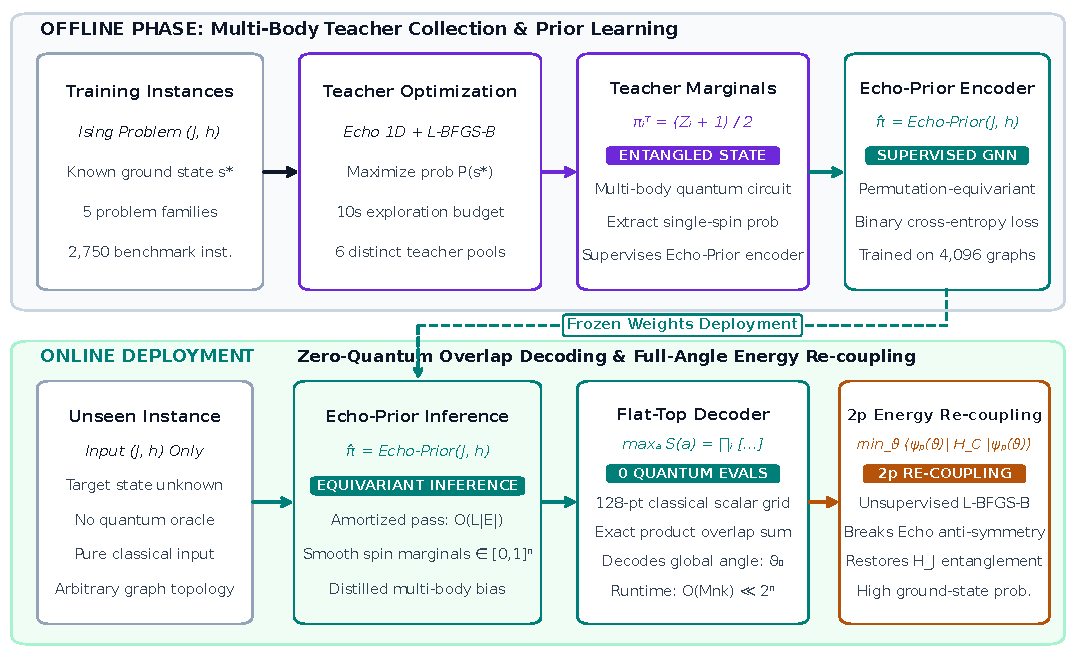
\includegraphics[width=0.86\textwidth]{figures/fig1_echo_qaoa_overview.pdf}}
\vskip -0.06in
\caption{\textbf{Overview of Echo-QAOA and Echo-Prior.} \textbf{(A)} Offline distillation extracts smooth single-qubit spin marginals $\pi_i^{\mathrm T}$ from multi-body Echo teachers. \textbf{(B)} Complete Echo pairs cancel even-parity $H_J$ via global spin-flip conjugation $F$, yielding exact single-qubit responses $q_i(a)$. \textbf{(C)} Online deployment maps unseen $(J,h)$ (1) via frozen \texttt{Echo-Prior} weights to spin marginals $\hat{\pi}$ (2), decodes fault-tolerant Flat-Top starts $\vartheta_0$ with zero quantum measurements (3), and releases all $2p$ angles to reactivate $H_J$ entanglement under L-BFGS-B (4).}
\label{fig:1}
\end{center}
\vskip -0.18in
\end{figure*}

To break this bottleneck, our core insight is to \textbf{carve out an exact product submanifold with explicit single-qubit responses and interval convexity inside the standard QAOA circuit via parity decoupling, and use it as an analytical bridge to reformulate ill-conditioned global angle regression into well-conditioned node-level quantum marginal distillation}. Inspired by Spin Echo refocusing \citep{carr1954effects,hahn1950spin,viola1999dynamical}, we exploit the opposite parities of $H_J$ (even) and $H_h$ (odd) under the global spin flip $F=\prod_i X_i$ ($\beta=\pi/2$) to formulate \textbf{Echo-QAOA}: pairing anti-symmetric cost angles $(-g_j,g_j)$ with a $\pi/2$ flip cancels $H_J$ exactly, factorizing target probabilities into $O(kn)$ single-qubit responses. Isomorphic to polynomial synthesis in Quantum Signal Processing \citep{gilyen2019quantum,low2017optimal,low2016methodology}, this yields \textbf{Flat-Top}, \textbf{Alternating-Phase}, and \textbf{Endpoint-Matched} 1D recipes, where Daubechies spectral factorization guarantees $O(\delta^{2k})$ error tolerance and strict convexity on zero-free intervals \citep{daubechies1988orthonormal,herrmann1971approximation}. Product factorization reduces the inner product between $2^n$-D distributions to $n$ single-qubit marginal terms, yielding an $O(Mnk)$ \textbf{1D distribution-overlap decoder} with \textbf{zero online quantum evaluations}. Building on this decoder, \textbf{Echo-Prior} uses a permutation-equivariant message-passing network \citep{gilmer2017neural,karalias2020erdos,schuetz2022combinatorial,xu2019how} to distill single-qubit positive-spin marginals $\pi_i^{\mathrm T}\in[0,1]$ of multi-body teacher states \citep{hinton2015distilling,wainwright2008graphical} from raw $(J,h)$, decodes them into fault-tolerant Flat-Top starts, and releases all $2p$ angles in Stage 2 to reactivate $H_J$ entanglement (Figure 1). Our contributions are:

\begin{enumerate}\setlength{\itemsep}{0pt}\setlength{\parskip}{1pt}\setlength{\topsep}{1pt}
\item \textbf{Echo-Pair Parity Decoupling and Constructive 1D Recipes}: We prove exact $H_J$ cancellation and $O(kn)$ probability factorization for complete Echo pairs (Propositions 1--2); we formulate Flat-Top, Alternating-Phase, and Endpoint-Matched 1D recipes, proving via Daubechies spectral factorization that arbitrary-order Flat-Top responses admit real angles (Proposition 3), $O(\delta^{2k})$ error tolerance, and strict interval convexity (Proposition 4), alongside local-field boundaries and recoupling (Proposition 5; Section 3).
\item \textbf{Implicit-Function Diagnosis, Overlap Decoder, and Echo-Prior}: We prove the inverse curvature trade-off between peak flatness and coordinate stability alongside cross-branch jumping; we construct a zero-measurement 1D overlap decoder $S(a)$ and propose permutation-equivariant Per-Qubit Marginal Distillation (\texttt{Echo-Prior-Flat/\allowbreak{}End/\allowbreak{}Alt}), decoupling spin-marginal inference from non-convex angles (Section 4).
\item \textbf{2,750-Instance Benchmark, 36-Model Evaluation, and 5,120-Instance Cross-Scale Generalization}: Across 2,750 instances, Flat-Top Echo achieves the highest overall mean probability ($\mathbf{53.07}\%$), beating TQA by $+13.52\text{--}+17.03$ pp on MWIS and across all scales under uncapped convergence; on unseen MWIS instances, \textbf{Echo-Prior-Flat} achieves the highest cross-depth mean probability ($\mathbf{23.48}\%$) with zero Stage-1 measurements, expanding $P_{\mathrm{gs}}\ge 50\%$ coverage to $\mathbf{20.0}\%$ ($4.9\times$ GNN-TQA), beating all 36 angle-regression models and 1D pooled ablations, and generalizing zero-shot across $n\in\{6,8,10,12,14\}$ (5,120 instances) with $100\%$ Stage-1 noise immunity (Section 5).

\end{enumerate}
\section{Related Work}\label{sec:2}

\subsection{Constrained Ising Variational Optimization and Heuristic Trajectory Initialization}\label{subsec:2_1}

QAOA \citep{farhi2014quantum} discretizes adiabatic evolution \citep{farhi2001quantum,kadowaki1998quantum} into alternating parameterized circuits \citep{blekos2024review,cerezo2021variational,preskill2018quantum}. Penalty mappings \citep{lucas2014ising} and constrained ans\"atze \citep{hadfield2019quantum} map NP-hard problems like MWIS to Ising models with competing $J$ and heterogeneous fields $h$ across superconducting, trapped-ion, and Rydberg platforms \citep{ebadi2022quantum,harrigan2021quantum,pagano2020quantum,pichler2018quantum}. Direct $2p$-angle optimization faces barren plateaus \citep{mcclean2018barren}, NP-hard landscapes \citep{bittel2021training}, local traps \citep{anschuetz2022quantum,you2021exponentially}, and symmetries \citep{lotshaw2021empirical,shaydulin2021classical}, making multi-start quasi-Newton search \citep{byrd1995limited,shaydulin2019multistart} with $O(p)$ parameter-shift gradients \citep{mitarai2018quantum,wierichs2022general} costly. Heuristic schedules---interpolation/Fourier bases \citep{crooks2018performance,zhou2020quantum}, counterdiabatic driving \citep{wurtz2022counterdiabaticity,yang2017optimizing}, TQA \citep{sack2021quantum}, and parameter transfer \citep{brandao2018fixed,galda2021transferability,shaydulin2023parameter}---impose uniform phase envelopes that fail under heterogeneous fields $h$ \citep{katial2025instance}. Ansatz-modifying variants like Warm-Start QAOA \citep{egger2021warm,tate2023warm}, ma-QAOA \citep{herrman2022multi}, and RQAOA \citep{bravyi2020obstacles} alter initial states or mixers $U_B(\beta)$, forfeiting native global-pulse compatibility. We preserve the unmodified QAOA ansatz, carving out an exact 1D product submanifold before recoupling all $2p$ angles \citep{dupont2022entanglement}.

\subsection{Spin Echo, Quantum Signal Processing, and Daubechies Wavelet Spectral Factorization}\label{subsec:2_2}

Intermediate $\pi$ flips that reverse linear phase evolution underpin NMR Spin Echo \citep{carr1954effects,hahn1950spin}, dynamical decoupling \citep{viola1999dynamical}, and composite pulses \citep{vandersypen2005nmr}. In standard QAOA, $\beta=\pi/2$ implements the global spin flip $F=\prod_i X_i$ up to a global phase; pairing anti-symmetric cost angles $(-g_j,g_j)$ with $\beta=\pi/2$ cancels even-parity $H_J$ while doubling odd-parity $H_h$. Within the decoupled single-qubit subspace, synthesizing even-layer mixers $(\theta_1,\ldots,\theta_k)$ is isomorphic to polynomial spectral synthesis in QSP and QSVT \citep{gilyen2019quantum,low2017optimal,low2016methodology}. Importing maximally flat filters and Daubechies' power-complementary spectral factorization \citep{daubechies1988orthonormal,herrmann1971approximation}, we embed two-channel orthogonal lattice elimination into complete Echo pairs to guarantee real-angle realizability, $O(\delta^{2k})$ flatness, and interval convexity.

\subsection{Amortized Implicit-Function Trade-offs and Per-Qubit Marginal Distillation}\label{subsec:2_3}

For online initialization without target states, research has shifted from recurrent L2O controllers \citep{verdon2019learning} to direct angle prediction via MLPs, GNNs, or diffusion models \citep{amosy2024iteration,jain2022graph,jiang2025qseer,liang2024invited,meng2025conditional}. By implicit differentiation in amortized optimization \citep{amos2023tutorial,gould2021deep}, reducing peak curvature for error tolerance inversely amplifies coordinate sensitivity to instance perturbations, while zero-probability manifolds trigger cross-branch jumps; even with set losses \citep{rupprecht2017learning,zhang2019deep}, global graph pooling \citep{xu2019how} erases node-level field biases. Inspired by graphical-model marginal inference \citep{wainwright2008graphical} and equivariant graph solvers \citep{gilmer2017neural,karalias2020erdos,loshchilov2019decoupled,schuetz2022combinatorial}, we pair Echo-QAOA's overlap decoder with knowledge distillation \citep{hinton2015distilling} of a permutation-equivariant \textbf{Echo-Prior} network to bypass angle jumps.

\section{Echo-QAOA: Operator Decoupling and Constructive 1D Response Theory}\label{sec:3}

\subsection{Ising Circuit Conventions with Local Fields and Exact Complete Echo-Pair Decoupling}\label{subsec:3_1}

Consider an $n$-spin Ising energy $E(s)=\frac12s^\top Js+h^\top s+C$ over $s\in\{-1,+1\}^n$, with symmetric zero-diagonal coupling $J\in\mathbb R^{n\times n}$, external field $h\in\mathbb R^n$, and offset $C\in\mathbb R$. Promoting spins to computational-basis operators decomposes $H_C=H_J+H_h+C$, where $H_J|s\rangle=(\frac12s^\top Js)|s\rangle$ and $H_h|s\rangle=(h^\top s)|s\rangle$ ($C$ adds only a global phase). In a depth-$p$ QAOA circuit \citep{farhi2014quantum} with cost unitary $U_C(\gamma)=e^{-i\gamma H_C}$ and mixer $U_B(\beta)=e^{-i\beta\sum_{i=1}^n X_i}$, starting from $|+\rangle^{\otimes n}$ prepares $|\psi_p(\vartheta;J,h)\rangle=U_B(\beta_p)U_C(\gamma_p)\cdots U_B(\beta_1)U_C(\gamma_1)|+\rangle^{\otimes n}$, where $\vartheta=(\gamma_1,\ldots,\gamma_p,\beta_1,\ldots,\beta_p)$ satisfies $|\gamma_\ell|\le G, |\beta_\ell|\le\pi/2$.

While $H_J$ generates complex multi-body interference \citep{bravyi2020obstacles,herrman2022multi}, conjugating $H_J$ and $H_h$ by the \textbf{global spin-flip operator} $F=\prod_{i=1}^n X_i$ ($s\mapsto -s$) reveals opposite parities: $FH_JF=H_J$, $FH_hF=-H_h$, and $U_B(\pi/2)=(-i)^nF$. Inspired by Spin Echo refocusing \citep{carr1954effects,hahn1950spin,vandersypen2005nmr,viola1999dynamical}, for positive even depths $p=2k$ ($k\ge 1$), we group adjacent layers into the $j$-th \textbf{complete Echo pair} ($j=1,\ldots,k$) with $(\gamma_{2j-1},\gamma_{2j})=(-g_j,g_j)$ and $(\beta_{2j-1},\beta_{2j})=(\pi/2,\theta_j)$.

\begin{proposition}[Complete Echo-Pair Decoupling]
\label{prop:1}
Up to a global phase, the composite unitary evolution operator of the $j$-th complete Echo pair, $E(g_j,\theta_j):=U_B(\theta_j)U_C(g_j)U_B(\pi/2)U_C(-g_j)$, satisfies identically $E(g_j,\theta_j)=U_B(\theta_j)e^{-2ig_jH_h}F$.
\end{proposition}

\begin{proof}[Proof Sketch]
Using $U_B(\pi/2)\propto F$, $F^2=I$, $F(H_J+H_h+C)F=H_J-H_h+C$, and $[H_C,FH_CF]=0$ cancels $H_J$ and $C$ identically while doubling $-ig_jH_h$ across all $k$ pairs without weak-coupling approximations, preserving a strict product state from $|+\rangle^{\otimes n}$ (Appendix A.1).
\end{proof}

\begin{table*}[t]
\vskip -0.04in
\caption{Comparison of parameter designs, single-qubit responses, and theoretical properties across the three constructive Echo recipes ($p=2k, k\ge 2$, where $\phi=4ah$ and $t=\sin\phi$).}
\label{tab:1}
\vskip 0.01in
\centering
\footnotesize
\renewcommand{\arraystretch}{0.96}
\setlength{\tabcolsep}{4.0pt}
\resizebox{\textwidth}{!}{%
\begin{tabular}{>{\raggedright\arraybackslash}p{3.0cm}>{\raggedright\arraybackslash}p{5.0cm}>{\raggedright\arraybackslash}p{4.3cm}>{\raggedright\arraybackslash}p{7.8cm}}
\toprule
Recipe Name & Cost Ratios $r_j$ \& Even-Layer Mixers $\theta_j$ & Magnetization $m_k(t)$ \& Domain $\mathcal A_{v,k}$ & Core Algebraic and Analytical Properties \\
\midrule
\textbf{Flat-Top Echo} (\texttt{Echo-Flat}) & $r=(1,2,\ldots,2)$; $\theta_j$ via Daubechies spectral-factor elimination & $2I_{(1+t)/2}(k,k)-1$, $a\in[-\frac{G}{2},\frac{G}{2}]$ & Vanishing derivatives up to order $k-1$ at $t=\pm 1$ with $O(\delta^{2k})$ error tolerance; strictly convex on zero-free intervals \\
\textbf{Alternating-Phase Echo} (\texttt{Echo-Alt}) & $r_j=(-1)^{k-j}$; $\theta_j=0\ (j<k)$, $\theta_k=\pi/4$ & $\sin(k\phi)$, $a\in[-G,G]$ & Saturates cumulative phase bound $kG$ of zero-intermediate-mixer subfamily, expanding phase scanning frequency by $k\times$ \\
\textbf{Endpoint-Matched Echo} (\texttt{Echo-End}) & $r=(1,2,\ldots,2)$; $\theta_j=(-1)^{k-j}B\ (j<k)$, $\theta_k=B/2$ & $\sin[(2k-1)\arcsin(ut)]$, $a\in[-\frac{G}{2},\frac{G}{2}]$ & Balances passband endpoints $m_k(\tau)=m_k(1)$ on $[\tau,1]$, providing a conditional analytical probability lower bound \\
\bottomrule
\end{tabular}%
}
\vskip -0.02in
\end{table*}

\subsection{Single-Qubit Amplitude Recursion, Multiplicative Probability Factorization, and 1D Parameter Families}\label{subsec:3_2}

By Proposition 1, the $2^n$-D evolution reduces to $n$ decoupled 2D recursions. In the basis $(|s_i=-1\rangle,|s_i=+1\rangle)$ with $u_i^{(0)}=\frac{1}{\sqrt{2}}\binom{1}{1}$ and single-qubit mixer $M(\theta)=\binom{\cos\theta\ \ -i\sin\theta}{-i\sin\theta\ \ \cos\theta}$, the state $u_i^{(j)}=\big(u_{i,-}^{(j)}, u_{i,+}^{(j)}\big)^\top$ updates via spin swap $X_i$, field phase $e^{\pm 2ig_jh_i}$, and mixing $M(\theta_j)$ as $\binom{u_{i,-}^{(j)}}{u_{i,+}^{(j)}}=M(\theta_j)\binom{e^{2ig_jh_i}u_{i,+}^{(j-1)}}{e^{-2ig_jh_i}u_{i,-}^{(j-1)}}$ ($j=1,\ldots,k$), yielding final magnetization $m_i=|u_{i,+}^{(k)}|^2-|u_{i,-}^{(k)}|^2\in[-1,1]$.

\begin{proposition}[Multiplicative Probability Factorization]
\label{prop:2}
Under a depth-$p=2k$ circuit of $k$ complete Echo pairs, the measurement probability of any target spin configuration $s^\star\in\{-1,+1\}^n$ factorizes as $P(s^\star)=\prod_{i=1}^n\frac{1+s_i^\star m_i}{2}$.
\end{proposition}

\begin{proof}[Proof Sketch]
Product-state preservation makes qubit measurements independent with marginal $|u_{i,s_i^\star}^{(k)}|^2=(1+s_i^\star m_i)/2$ (Appendix A.1), reducing evaluation from $O(pn2^n)$ to $O(kn)$ time and $O(1)$ space.
\end{proof}

For even depth $p=2k$ and recipe $v$, fixing cost ratios $(r_1,\ldots,r_k)$ and even-layer mixers $(\theta_1,\ldots,\theta_k)$ drives all cost amplitudes via a single scalar $a$ ($g_j=r_ja$) through the affine embedding $D_{v,k}(a)=(-r_1a,r_1a,\ldots,-r_ka,r_ka,\tfrac\pi2,\theta_1,\ldots,\tfrac\pi2,\theta_k)$ over $a\in\mathcal A_{v,k}=[-G/\max_j|r_j|,G/\max_j|r_j|]$, where $m_i(a)$ depends only on $\phi_i=4ah_i$ and $(r_j,\theta_j)_{j=1}^k$.


\subsection{Flat-Top Echo: High-Order Flat Response and Spectral-Factor Realizability}\label{subsec:3_3}

Because site fields $h_i$ are generally incommensurate, a single scalar $a$ cannot align every qubit at $\sin(4ah_i)=s_i^\star$. \textbf{Flat-Top Echo} adopts the dyadic ratio $r=(1,2,\ldots,2)$ ($a\in[-G/2,G/2]$ for $k\ge 2$) and shapes the single-qubit magnetization in $t=\sin(4ah)\in[-1,1]$ via the normalized symmetric Beta integral $m_k(t)=\int_0^t(1-z^2)^{k-1}\,dz/\int_0^1(1-z^2)^{k-1}\,dz$, with success factor $p_k(q)=(1+m_k(2q-1))/2=I_q(k,k)$ for $q=(1+t)/2\in[0,1]$ and $p_k(q)+p_k(1-q)=1$ (e.g., $m_2(t)=(3t-t^3)/2$ and $m_3(t)=(15t-10t^3+3t^5)/8$; Appendix A.2). Here $m_k(t)$ is an odd degree-$(2k-1)$ polynomial satisfying $m_k(\pm 1)=\pm 1$ with derivatives of order $1\ldots k-1$ vanishing at $t=\pm 1$.

\begin{proposition}[Constructive Realizability of Arbitrary-Order Flat-Top Responses]
\label{prop:3}
For any integer $k\ge 1$, there exist real angles $\theta_1,\ldots,\theta_k\in[-\pi/2,\pi/2)$ such that a $k$-pair complete Echo circuit with cost ratios $g=(a,2a,\ldots,2a)$ produces the exact single-qubit magnetization response $m_k(\sin(4ah))$.
\end{proposition}

\begin{proof}[Construction and Proof Sketch]
Setting $\omega=4ah-\pi/2$ and $z=e^{i\omega}$ ($q=\cos^2(\omega/2)$), Daubechies' power-complementary spectral factorization \citep{daubechies1988orthonormal,herrmann1971approximation} yields a real minimum-phase polynomial $H_k(z)=\sum_{r=0}^{2k-1}c_rz^r$ satisfying $|H_k(e^{i\omega})|^2/2=p_k(\cos^2(\omega/2))$ and $|H_k(z)|^2+|H_k(-z)|^2=2$. Pairing $H_j(z)$ with $H_j^\#(z)=z^{2j-1}H_j(-z^{-1})$, two-channel orthogonal lattice elimination from $j=k$ to $1$ cancels constant and linear terms at each step (divisible by $e^{2i\phi}=-z^2$) to extract unique real angles $\theta_j\in[-\pi/2,\pi/2)$ whose reverse recursion matches Section 3.2 (Appendix A.2).
\end{proof}

Around peak alignment $s_i^\star\sin(4a_0h_i)=1$, a perturbation $a=a_0+\delta$ gives $1-s_i^\star\sin(4h_i(a_0+\delta))=8h_i^2\delta^2+O(\delta^4)$. Since $1-m_k(1-\varepsilon)=O(\varepsilon^k)$, single-qubit probability loss is suppressed to $O(\delta^{2k})$, widening each qubit's high-probability overlap window under incommensurate fields.

\begin{figure*}[t]
\vskip -0.02in
\begin{center}
\centerline{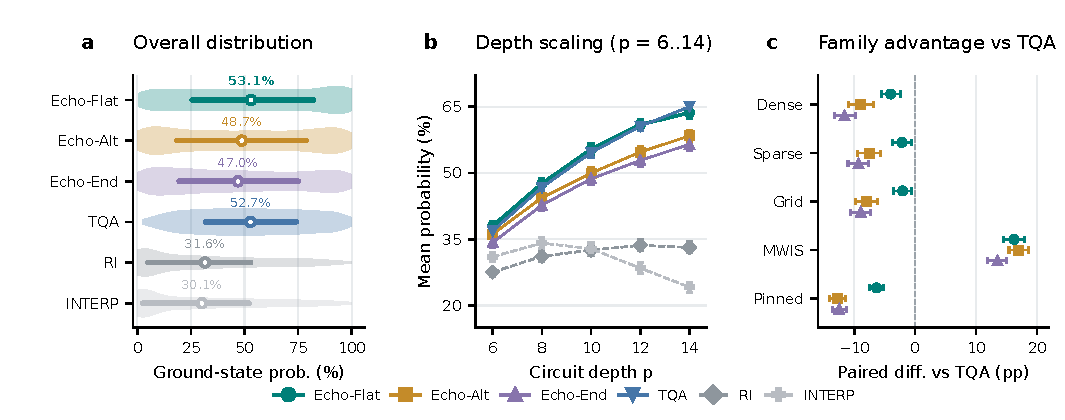
\includegraphics[width=0.74\textwidth]{figures/benchmark-comparison.pdf}}
\vskip -0.06in
\caption{\textbf{Constructive initialization and probability optimization across the five-family benchmark (2,750 instances, $n=6\ldots 16, p\in\{6,8,10,12,14\}$).} (a) Violin plots, interquartile ranges, and mean markers of overall ground-state probability across five depths and all 2,750 instances; (b) Mean ground-state probability scaling curves across depths $p=6\ldots 14$ (with 95\% CIs); (c) Per-instance paired probability differences (pp) of the three Echo recipes relative to TQA across the five families (550 instances per family).}
\label{fig:2}
\end{center}
\vskip -0.24in
\end{figure*}

\begin{table*}[t]
\vskip -0.04in
\caption{Mean ground-state probabilities by problem family and overall across the five-family benchmark (550 instances per family, 2,750 total; unit: \%). Superscripts and subscripts denote 95\% bootstrap CI offsets (pp); row maxima are in bold.}
\label{tab:2}
\vskip 0.01in
\centering
\footnotesize
\renewcommand{\arraystretch}{0.96}
\setlength{\tabcolsep}{4.0pt}
\resizebox{0.78\textwidth}{!}{%
\begin{tabular}{lcccccc}
\toprule
Problem Family & \texttt{Echo-Flat} & \texttt{Echo-Alt} & \texttt{Echo-End} & RI & TQA & INTERP \\
\midrule
Dense Ising & $56.17^{+2.39}_{-2.57}$ & $51.27^{+2.59}_{-2.73}$ & $48.57^{+2.50}_{-2.58}$ & $27.47^{+2.18}_{-2.12}$ & $\mathbf{60.18}^{+1.83}_{-1.88}$ & $30.36^{+2.42}_{-2.43}$ \\
Sparse Ising & $60.16^{+2.34}_{-2.45}$ & $54.84^{+2.49}_{-2.68}$ & $53.02^{+2.44}_{-2.57}$ & $32.92^{+2.31}_{-2.32}$ & $\mathbf{62.33}^{+1.82}_{-1.90}$ & $30.84^{+2.39}_{-2.47}$ \\
Grid Ising & $60.64^{+2.37}_{-2.44}$ & $54.73^{+2.57}_{-2.60}$ & $53.74^{+2.50}_{-2.58}$ & $35.75^{+2.45}_{-2.52}$ & $\mathbf{62.69}^{+1.95}_{-1.91}$ & $33.82^{+2.51}_{-2.54}$ \\
MWIS & $49.34^{+2.85}_{-2.93}$ & $\mathbf{50.09}^{+2.62}_{-2.75}$ & $46.59^{+2.63}_{-2.73}$ & $38.46^{+2.58}_{-2.67}$ & $33.07^{+1.77}_{-1.79}$ & $31.64^{+2.36}_{-2.52}$ \\
Pinned MaxCut & $39.06^{+2.21}_{-2.22}$ & $32.63^{+2.21}_{-2.21}$ & $32.94^{+2.09}_{-2.08}$ & $23.33^{+1.92}_{-1.91}$ & $\mathbf{45.39}^{+1.95}_{-1.85}$ & $23.91^{+2.10}_{-2.12}$ \\
\textbf{Overall Mean (2,750 inst.)} & $\mathbf{53.07}^{+1.15}_{-1.18}$ & $48.71^{+1.20}_{-1.20}$ & $46.97^{+1.14}_{-1.17}$ & $31.59^{+1.06}_{-1.07}$ & $52.73^{+0.93}_{-0.95}$ & $30.11^{+1.07}_{-1.11}$ \\
\bottomrule
\end{tabular}%
}
\vskip -0.02in
\end{table*}

\subsection{Strict Convexity of the Flat-Top Objective on Zero-Free Intervals}\label{subsec:3_4}

For target $s^\star$, let $w_i=4h_is_i^\star$ and define wrapped phase deviation $e_i(a)=\operatorname{wrap}_{(-\pi,\pi]}(aw_i-\pi/2)$. The negative log-probability loss of Flat-Top Echo decomposes into per-qubit phase losses $\mathcal L_k(a;x)=-\log P_{D_{\mathrm{flat},k}(a)}(s^\star)=\sum_{i=1}^n \ell_k(e_i(a))$, where $\ell_k(e):=-\log p_k((1+\cos e)/2)$.

\begin{proposition}[Strict Convexity on Zero-Free Intervals]
\label{prop:4}
The single-qubit phase loss $\ell_k(e)$ is strictly convex on $(-\pi,\pi)$. For any instance with at least one non-zero local field ($h_i\ne 0$), the global loss $\mathcal L_k(a;x)$ is strictly convex in $a$ on every open scalar interval free of zero-probability singularities, admitting at most one stationary point (its unique local minimum) per interval.
\end{proposition}

\begin{proof}[Proof Sketch]
Writing $p_k((1+\cos e)/2)=\int_e^\pi\sin^{2k-1}v\,dv/\int_0^\pi\sin^{2k-1}v\,dv$ for $e\in[0,\pi)$, strict log-concavity of $\sin^{2k-1}v$ on $(0,\pi)$ implies a strictly decreasing Mills tail ratio $R(e)$, making $\ell_k'(e)=1/R(e)$ strictly increasing on $(-\pi,\pi)$. Within any open interval avoiding zero-probability breakpoints $a=(-\pi/2+2\pi z)/w_i$ ($z\in\mathbb Z, w_i\ne 0$), each $e_i(a)$ is strictly affine in $a$, preserving strict convexity under summation (Appendix A.3).
\end{proof}

\subsection{Alternating-Phase Echo: Cumulative Effective Phase Expansion}\label{subsec:3_5}

To maximize cumulative phase range under $|g_j|\le G$, \textbf{Alternating-Phase Echo} ($k\ge 2$) sets $g_j=(-1)^{k-j}a$, $\theta_j=0$ ($j<k$), and $\theta_k=\pi/4$. Because intermediate flips $F$ invert accumulated local-field phases ($A_j=g_j-A_{j-1}$), alternating signs accumulate constructively to $A_k=ka$, saturating the subfamily bound $|A_k|\le\sum_{j=1}^k|g_j|\le kG$ and yielding $m_i(a)=\sin(4kah_i)$ (Appendix A.1).

\subsection{Endpoint-Matched Echo: Positive-Phase Passband Balancing and Recipe Comparison}\label{subsec:3_6}

Balancing flatness and oscillation, \textbf{Endpoint-Matched Echo} ($k\ge 2$) retains $g=(a,2a,\ldots,2a)$ ($a\in[-G/2,G/2]$) with alternating mixers $\theta_j=(-1)^{k-j}B$ ($j<k$) and $\theta_k=B/2$. Grouping adjacent pairs into coaxial Bloch rotations with $L=2k-1$, $u=\sin B$, and $t=\sin(4ah)$ \citep{low2016methodology,vandersypen2005nmr} (Appendix A.4) yields $m_k(t)=\sin[L\arcsin(ut)]$. For passband threshold $\tau\in(0,1)$, setting $u=\sin(\pi/L)/\sqrt{1+2\tau\cos(\pi/L)+\tau^2}$ and $B=\arcsin u$ enforces $m_k(\tau)=m_k(1)$, ensuring $P_{D_{\mathrm{end},k}(a)}(s^\star)\ge[(1+m_k(\tau))/2]^n$ when all $t_i=s_i^\star\sin(4ah_i)\in[\tau,1]$ (Table 1).

\subsection{Theoretical Boundaries of Restricted Product Evolution and Motivation for Recoupling}\label{subsec:3_7}

Because complete Echo pairs cancel $H_J$ exactly, Stage-1 evolution is driven purely by $H_h$, establishing structural bounds that motivate Stage-2 full-angle recoupling.

\begin{proposition}[Local-Field-Driven Boundaries and Multiplicative Decay of Restricted Echo Evolution]
\label{prop:5}
Under the depth-$p=2k$ restricted Echo circuit $D_{v,k}(a)$, target probability obeys:
(1) \textbf{Zero-Field Upper Bound}: If $n_0$ qubits have $h_i=0$, then $P_{D_{v,k}(a)}(s^\star)\le 2^{-n_0}$ for all $a$ (reducing to $2^{-n}$ when $h=0$);
(2) \textbf{Dimensional Attenuation Bound}: If $q$ qubits have $s_i^\star m_i(a)\le\eta<1$ at scalar $a$, then $P_{D_{v,k}(a)}(s^\star)\le\big(\frac{1+\eta}{2}\big)^q$.
\end{proposition}

\begin{proof}[Proof Sketch]
Qubits with $h_i=0$ accumulate trivial phase on $|+\rangle$, fixing $m_i(a)=0$ and factor $1/2$ in Proposition 2; qubits with $s_i^\star m_i(a)\le\eta$ contribute $\le(1+\eta)/2$ (Appendix A.1).
\end{proof}

To resolve zero-field sites and frustrated couplings beyond product states, perturbing the $j$-th pair's cost angles along the symmetry-breaking direction to $(-g_j+\delta_j, g_j+\delta_j)$ yields $U_B(\theta_j)e^{-2i\delta_j H_J}e^{-2ig_j H_h}F$ (Appendix A.1), reactivating the coupling generator $H_J$ linearly at $O(\delta_j)$ and inducing non-zero energy gradients under non-degenerate even-layer mixers ($\theta_j\notin\{0,\pm\pi/2\}$). This establishes Echo-QAOA's \textbf{two-stage division of labor} \citep{dupont2022entanglement,wurtz2022counterdiabaticity,yang2017optimizing}: Stage 1 anchors a field-aligned starting point on the 1D Echo manifold in $O(kn)$ classical time; Stage 2 releases all $2p$ angles to restore entanglement.

\subsection{1D Interval Derivative Root-Finding and Two-Stage Optimization Strategy}\label{subsec:3_8}

For offline teacher collection with known $s^\star$ (Appendix B.1), Stage 1 locates 1D candidates via: (1) deterministic bisection on $\mathcal L_k'(a;x)$ within each zero-free convex interval (Proposition 4) for Flat-Top Echo; (2) $O(kn)$ grid peak-finding with golden-section refinement for oscillatory recipes; and (3) spacing deduplication before Stage-2 L-BFGS-B refinement.

\section{Per-Qubit Marginal Distillation Initialization via Distribution-Overlap Decoding}\label{sec:4}

\begin{figure*}[t]
\vskip -0.02in
\begin{center}
\centerline{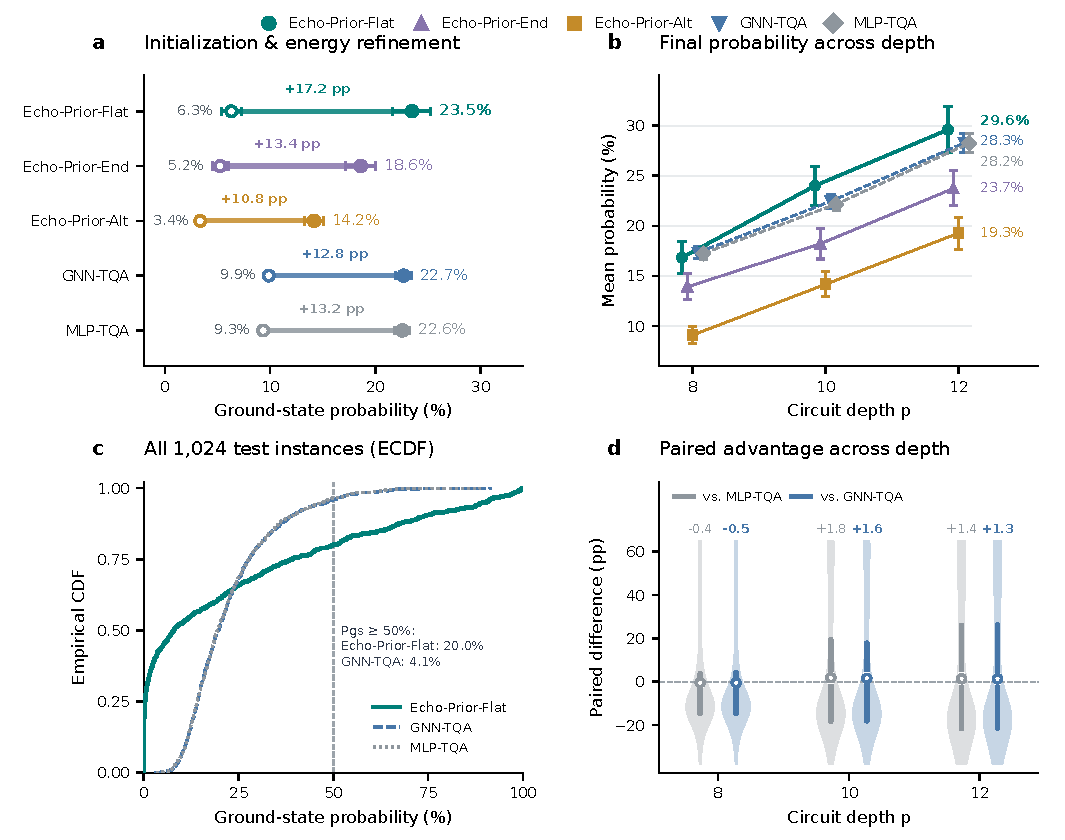
\includegraphics[width=0.58\textwidth]{figures/neural-n10.pdf}}
\vskip -0.06in
\caption{\textbf{Comparison of per-qubit quantum teacher distillation (Echo-Prior) and full-angle regression models on unseen MWIS test instances ($n=10$, 1,024 instances).} (a) Dumbbell plot of cross-depth initial (open circles) and post-L-BFGS-B final ground-state probability (filled circles), annotated with net energy-recoupling gains (pp); (b) Final mean probability scaling across $p=8,10,12$; (c) ECDFs of cross-depth mean final probability and high-probability coverage ($P_{\mathrm{gs}}\ge 50\%$); (d) Violin plots of per-instance paired net gains of Echo-Prior-Flat over MLP-TQA and GNN-TQA.}
\label{fig:3}
\end{center}
\vskip -0.24in
\end{figure*}

\subsection{Local Sensitivity Trade-offs and Cross-Branch Jumping in Parameter Space}\label{subsec:4_1}

To design a cross-instance generator from $x=(J,h)$ to $\vartheta^\star(x)$ \citep{amos2023tutorial,verdon2019learning}, let $a_b^\star(x)\in I_b(x)$ be the unique interior stationary point ($\partial_a\mathcal L_k(a_b^\star(x);x)=0$) on a zero-free Flat-Top branch $I_b(x)$ with curvature $\partial_{aa}\mathcal L_k\ge\mu>0$ and $\|\partial_{ax}\mathcal L_k\|\le M$. By the implicit function theorem \citep{amos2023tutorial,gould2021deep}, label sensitivity satisfies $\nabla_xa_b^\star(x)=-(\partial_{aa}\mathcal L_k(a_b^\star;x))^{-1}\partial_{ax}\mathcal L_k(a_b^\star;x)$ (bounded by $M/\mu$), while under prediction error $\delta=\widehat a-a_b^\star$ the loss increases as $\Delta\mathcal L_k(\delta;x)=\frac12\mathcal L_k''(a_b^\star;x)\delta^2+o(\delta^2)$. Under heterogeneous fields where aligned qubits sit on the flat top (diluting total restoring curvature $\mathcal L_k''$) while off-peak qubits retain non-zero cross-derivatives $\partial_{ax}\mathcal L_k\ne 0$, this exposes a conditional \textbf{curvature--sensitivity trade-off}: flattening the peak tolerates larger errors $\delta$ ($O(\delta^{2k})$ at ideal alignment), yet amplifies local coordinate drift $(\partial_{aa}\mathcal L_k)^{-1}\partial_{ax}\mathcal L_k$. Globally, zero-probability breakpoints partition $\mathcal A_{v,k}$ into competing branches $\{I_b(x)\}$ whose crossings trigger discontinuous jumps in $a^\star(x)$, while sign and periodic symmetries collapse direct angle regression toward low-overlap averages (Appendix A.3). We therefore infer a symmetry-invariant, bounded \textbf{single-qubit positive-spin marginal prior} $\boldsymbol{\pi}=(\pi_1,\ldots,\pi_n)\in[0,1]^n$ in state space and project it analytically onto the Echo manifold.

\subsection{1D Distribution-Overlap Decoding and Full-Angle Energy Recoupling}\label{subsec:4_2}

Given an estimated marginal prior $\boldsymbol{\pi}\in[0,1]^n$ defining the surrogate product distribution $P_{\pi}(s)=\prod_{i=1}^n\pi_i^{\mathbf1[s_i=+1]}(1-\pi_i)^{\mathbf1[s_i=-1]}$, Proposition 2 guarantees that the restricted Echo distribution $Q_a(s)$ at scalar $a$ is also a strict product distribution with $+1$ marginal $q_i(a)=(1+m_i(a))/2$. Consequently, the $2^n$-D \textbf{Distribution Overlap} $S(a)=\sum_{s\in\{-1,+1\}^n}P_{\pi}(s)Q_a(s)=\prod_{i=1}^n[\pi_iq_i(a)+(1-\pi_i)(1-q_i(a))]$ factorizes into $n$ single-qubit terms. Evaluating $S(a)$ on an $M$-point uniform grid $\mathcal A_M\subset\mathcal A_{v,k}$ selects $\widehat a=\arg\max_{a\in\mathcal A_M}S(a)$ and expands $\vartheta_0=D_{v,k}(\widehat a)$ in $O(Mnk)$ classical time with \textbf{strictly zero Stage-1 online quantum evaluations}. Stage 2 then minimizes the unsupervised quantum energy $\min_{\vartheta}\langle\psi_p(\vartheta;J,h)|\frac12s^\top Js+h^\top s|\psi_p(\vartheta;J,h)\rangle$ via bound-constrained L-BFGS-B \citep{byrd1995limited}, driving all $2p$ angles off the anti-symmetric manifold to reactivate $H_J$ within the standard QAOA ansatz (Appendix B.1, D.2).

\begin{table*}[t]
\vskip -0.04in
\caption{Initial $\rightarrow\allowbreak$ post-energy-optimization mean ground-state probabilities (\%) on the MWIS test set ($n=10$, 1,024 instances) comparing online heuristics, representative $2p$-angle regression models (matched \texttt{Flat} vs. best \texttt{TQA} teachers; full 36-model breakdown in Table D.4), and per-qubit marginal distillation (\texttt{Echo-Prior}). Best values are in bold.}
\label{tab:3}
\vskip 0.01in
\centering
\footnotesize
\renewcommand{\arraystretch}{0.96}
\setlength{\tabcolsep}{5.5pt}
\resizebox{0.94\textwidth}{!}{%
\begin{tabular}{llccccc}
\toprule
Paradigm & Method & Stage-1 Evals & $p = 8$ & $p = 10$ & $p = 12$ & Cross-Depth Mean \\
\midrule
\textbf{Online Heuristics} & \textbf{RI (1)} & $0$ & $0.10 \rightarrow\allowbreak 3.84^{+0.60}_{-0.57}$ & $0.10 \rightarrow\allowbreak 6.82^{+0.90}_{-0.87}$ & $0.10 \rightarrow\allowbreak 10.42^{+1.23}_{-1.20}$ & $7.03\%$ \\
 & \textbf{RI (32)} & $32$ & $0.22 \rightarrow\allowbreak 6.47^{+0.62}_{-0.60}$ & $0.20 \rightarrow\allowbreak 9.93^{+0.87}_{-0.81}$ & $0.17 \rightarrow\allowbreak 12.81^{+1.02}_{-0.97}$ & $9.73\%$ \\
 & \textbf{TQA} & $32$ & $4.60 \rightarrow\allowbreak 17.05^{+0.56}_{-0.56}$ & $6.81 \rightarrow\allowbreak 21.94^{+0.68}_{-0.68}$ & $8.23 \rightarrow\allowbreak 28.27^{+0.92}_{-0.91}$ & $22.42\%$ \\
\midrule
\textbf{Full-Angle Regression} & \textbf{MLP-Flat} & $0$ & $0.10 \rightarrow\allowbreak 4.52^{+0.71}_{-0.67}$ & $0.11 \rightarrow\allowbreak 7.98^{+1.07}_{-1.01}$ & $0.11 \rightarrow\allowbreak 11.73^{+1.37}_{-1.30}$ & $8.08\%$ \\
 & \textbf{MLP-TQA} & $0$ & $8.58 \rightarrow\allowbreak 17.24^{+0.61}_{-0.62}$ & $9.08 \rightarrow\allowbreak 22.17^{+0.68}_{-0.67}$ & $10.36 \rightarrow\allowbreak 28.25^{+0.93}_{-0.95}$ & $22.55\%$ \\
 & \textbf{GNN-Flat} & $0$ & $0.09 \rightarrow\allowbreak 4.19^{+0.69}_{-0.62}$ & $0.12 \rightarrow\allowbreak 7.04^{+1.00}_{-0.96}$ & $0.11 \rightarrow\allowbreak 10.06^{+1.33}_{-1.22}$ & $7.10\%$ \\
 & \textbf{GNN-TQA} & $0$ & $9.27 \rightarrow\allowbreak \mathbf{17.33}^{+0.60}_{-0.60}$ & $10.40 \rightarrow\allowbreak 22.45^{+0.70}_{-0.71}$ & $9.95 \rightarrow\allowbreak 28.28^{+0.94}_{-0.97}$ & $22.68\%$ \\
\midrule
\textbf{Per-Qubit Distillation} \emph{(Ours)} & \textbf{Echo-Prior-Alt} & $0$ & $3.46 \rightarrow\allowbreak 9.09^{+0.90}_{-0.85}$ & $3.32 \rightarrow\allowbreak 14.16^{+1.26}_{-1.26}$ & $3.30 \rightarrow\allowbreak 19.27^{+1.59}_{-1.61}$ & $14.18\%$ \\
 & \textbf{Echo-Prior-End} & $0$ & $5.21 \rightarrow\allowbreak 13.90^{+1.35}_{-1.28}$ & $5.22 \rightarrow\allowbreak 18.21^{+1.54}_{-1.52}$ & $5.31 \rightarrow\allowbreak 23.72^{+1.81}_{-1.70}$ & $18.61\%$ \\
 & \textbf{Echo-Prior-Flat} & $\mathbf{0}$ & $6.00 \rightarrow\allowbreak 16.83^{+1.59}_{-1.62}$ & $6.26 \rightarrow\allowbreak \mathbf{24.00}^{+1.93}_{-1.99}$ & $6.68 \rightarrow\allowbreak \mathbf{29.60}^{+2.27}_{-2.26}$ & $\mathbf{23.48}\%$ \\
\bottomrule
\end{tabular}%
}
\vskip -0.02in
\end{table*}

\subsection{Offline Probability Teachers and Symmetry-Aware Multi-Branch Angle-Set Supervision}\label{subsec:4_3}

On the training set (with known unique $s^\star$), we run the three Echo recipes and three baselines (RI, TQA, INTERP) to form six offline teachers. Retaining candidates within $\alpha_{\mathrm{prob}}\in(0,1)$ of each pool's peak probability, we account for sign inversion ($\vartheta\mapsto -\vartheta$) and $\pi$-periodicity of mixers \citep{lotshaw2021empirical,shaydulin2021classical} via the \textbf{normalized symmetry-equivalent distance} $d^2(\vartheta,\vartheta')=\min_{\sigma\in\{\pm 1\}}\frac{1}{2p}\sum_{\ell=1}^p\big[(\frac{\gamma_\ell-\sigma\gamma'_\ell}{G})^2+(\frac{\operatorname{wrap}_{\pi}(\beta_\ell-\sigma\beta'_\ell)}{\pi/2})^2\big]$. Greedy filtering with separation $d^2>\delta_{\mathrm{sep}}^2$ yields up to $R$ separated branches $\mathcal T_q=\{\vartheta_{qr}^{\mathrm T}\}_{r=1}^{R_q}$ per instance $q$. Full-angle regression baselines (MLPs and GNNs) \citep{amosy2024iteration,jain2022graph,liang2024invited} minimize the set loss $\mathcal L_q=\min_{\vartheta^{\mathrm T}\in\mathcal T_q}d^2(\widehat\vartheta_q,\vartheta^{\mathrm T})$ \citep{rupprecht2017learning,zhang2019deep}.

\subsection{Permutation-Equivariant Per-Qubit Teacher Marginal Learning (Echo-Prior)}\label{subsec:4_4}

To bypass angle-space discontinuities while distilling multi-body entanglement biases, \textbf{Echo-Prior} extracts single-qubit positive-spin marginals $\pi_i^{\mathrm T}=\sum_{s}|\langle s|\psi_p(\vartheta^{\mathrm T};J,h)\rangle|^2\mathbf1[s_i=+1]\in[0,1]$ from the top teacher state $\vartheta^{\mathrm T}\in\mathcal T_q$ \citep{hinton2015distilling}. Receiving only standardized raw coefficients $(\tilde J,\tilde h)$, the encoder embeds $\boldsymbol z_i^{(0)}=\phi_{\mathrm{node}}(\tilde h_i)\in\mathbb R^W$ and executes $L$ message-passing rounds over non-zero edges $M_{ij}=\mathbf1[J_{ij}\ne 0]$ \citep{gilmer2017neural,xu2019how}: $\boldsymbol a_i^{(\ell)}=\frac{1}{Z_{\mathrm{agg}}}\sum_{j=1}^n M_{ij}\,\phi_{\mathrm{msg}}^{(\ell)}(\boldsymbol z_i^{(\ell-1)},\boldsymbol z_j^{(\ell-1)},\tilde J_{ij})$ and $\boldsymbol z_i^{(\ell)}=\boldsymbol z_i^{(\ell-1)}+\phi_{\mathrm{upd}}^{(\ell)}(\boldsymbol z_i^{(\ell-1)},\boldsymbol a_i^{(\ell)})$ with fixed scale $Z_{\mathrm{agg}}$, outputting $\widehat\pi_i=\operatorname{sigmoid}(\phi_{\mathrm{head}}(\boldsymbol z_i^{(L)}))$ \citep{karalias2020erdos,schuetz2022combinatorial}. Shared edge/node parameters and topological aggregation guarantee strict \textbf{permutation equivariance}. We minimize per-qubit binary cross-entropy $\mathcal L_{\mathrm{BCE}}=-\frac{1}{|B|n}\sum_{q\in B,i}[\pi_{qi}^{\mathrm T}\log\widehat\pi_{qi}+(1-\pi_{qi}^{\mathrm T})\log(1-\widehat\pi_{qi})]$ and decode $\widehat{\boldsymbol{\pi}}$ via $S(a)$ (\textbf{Echo-Prior-Flat/End/Alt}) followed by full-angle L-BFGS-B refinement (Appendix B.3).

\section{Experiments}\label{sec:5}

\begin{table*}[t]
\vskip -0.04in
\caption{Controlled ablation of neural readout representations within the 1D Flat-Top Echo manifold on the MWIS test set ($n=10$, 1,024 instances; initial $\rightarrow\allowbreak$ post-optimization ground-state probability, \%).}
\label{tab:4}
\vskip 0.01in
\centering
\footnotesize
\renewcommand{\arraystretch}{0.96}
\setlength{\tabcolsep}{5.5pt}
\resizebox{0.86\textwidth}{!}{%
\begin{tabular}{llcccc}
\toprule
Method & Readout Representation & $p = 8$ & $p = 10$ & $p = 12$ & Mean \\
\midrule
\textbf{Echo-GNN-Scalar} & Directed 1D scalar $a_{\mathrm{dec}}$ (mean pool) & $0.26 \rightarrow\allowbreak 5.22^{+0.72}_{-0.66}$ & $0.27 \rightarrow\allowbreak 8.03^{+1.04}_{-0.93}$ & $0.29 \rightarrow\allowbreak 12.15^{+1.24}_{-1.17}$ & $8.47\%$ \\
\textbf{Echo-GNN-Grid} & 128-way soft grid (4th-moment pool) & $3.37 \rightarrow\allowbreak 11.63^{+1.35}_{-1.29}$ & $3.27 \rightarrow\allowbreak 16.53^{+1.58}_{-1.63}$ & $3.38 \rightarrow\allowbreak 22.55^{+1.91}_{-1.88}$ & $16.90\%$ \\
\textbf{Echo-Prior-Flat} & Per-qubit marginals $\hat{\pi}\in[0,1]^n$ & $\mathbf{6.00} \rightarrow\allowbreak \mathbf{16.83}^{+1.59}_{-1.62}$ & $\mathbf{6.26} \rightarrow\allowbreak \mathbf{24.00}^{+1.93}_{-1.99}$ & $\mathbf{6.68} \rightarrow\allowbreak \mathbf{29.60}^{+2.27}_{-2.26}$ & $\mathbf{23.48}\%$ \\
\bottomrule
\end{tabular}%
}

\vskip 0.02in
\caption{End-to-end two-point shifted-circuit optimization ($n=10, p=10$, 1,024 MWIS instances, $\delta=0.10$ rad; $1+41t$ Stage-2 evaluations: $657, 1{,}313, 2{,}625$ for \texttt{Echo-Prior-Flat} vs. $32+2{,}625=2{,}657$ for \texttt{TQA}; $\infty$ rows give matched Adam and L-BFGS-B references, \%).}
\label{tab:5}
\vskip 0.01in
\centering
\footnotesize
\renewcommand{\arraystretch}{0.96}
\setlength{\tabcolsep}{5.5pt}
\resizebox{0.88\textwidth}{!}{%
\begin{tabular}{cccccc}
\toprule
$N_{\mathrm{shots}}$ & Echo-Prior (16 steps) & Echo-Prior (32 steps) & Echo-Prior (64 steps) & TQA (64 steps) & Gain vs. TQA (pp) \\
\midrule
$64$ & $11.15^{+1.31}_{-1.28}$ & $13.46^{+1.45}_{-1.43}$ & $\mathbf{15.17}^{+1.56}_{-1.55}$ & $14.63^{+0.49}_{-0.50}$ & $+0.53\ ([-0.98, +2.01])$ \\
$256$ & $12.96^{+1.43}_{-1.47}$ & $15.78^{+1.62}_{-1.61}$ & $\mathbf{17.48}^{+1.69}_{-1.68}$ & $16.97^{+0.57}_{-0.56}$ & $+0.51\ ([-1.09, +2.12])$ \\
$1{,}024$ & $14.16^{+1.53}_{-1.52}$ & $16.90^{+1.67}_{-1.65}$ & $\mathbf{18.78}^{+1.74}_{-1.74}$ & $18.33^{+0.63}_{-0.62}$ & $+0.45\ ([-1.24, +2.17])$ \\
$4{,}096$ & $14.66^{+1.56}_{-1.56}$ & $17.56^{+1.71}_{-1.69}$ & $\mathbf{19.33}^{+1.80}_{-1.75}$ & $18.93^{+0.64}_{-0.63}$ & $+0.41\ ([-1.31, +2.15])$ \\
$\infty$ (Adam) & $14.85^{+1.57}_{-1.57}$ & $18.06^{+1.74}_{-1.71}$ & $\mathbf{19.61}^{+1.80}_{-1.80}$ & $19.32^{+0.66}_{-0.65}$ & $+0.28\ ([-1.41, +2.04])$ \\
$\infty$ (L-BFGS-B) & --- & --- & $\mathbf{24.00}^{+1.93}_{-1.99}$ & $21.94^{+0.68}_{-0.68}$ & $\mathbf{+2.06}\ ([+0.16, +3.97])$ \\
\bottomrule
\end{tabular}%
}
\vskip -0.10in
\end{table*}

\subsection{Experimental Setup and Evaluation Protocol}\label{subsec:5_1}

\textbf{Five-family offline benchmark.} We evaluate five problem families---fully connected \texttt{Dense Ising}, Hamiltonian-cycle \texttt{Sparse Ising}, 2D \texttt{Grid Ising}, single-spin-pinned \texttt{Pinned MaxCut}, and constrained \texttt{MWIS} with heterogeneous positive fields $h_i>0$ (protocols and uniqueness verification in Appendix C)---with 50 unique-ground-state instances per scale across $n\in\{6,\ldots,16\}$ (2,750 instances). Across $p\in\{6,8,10,12,14\}$, we compare \texttt{Echo-Flat}, \texttt{Echo-Alt}, \texttt{Echo-End}, \texttt{RI}, \texttt{TQA}, and \texttt{INTERP} under a 30.0 s wall-clock cap per task and uncapped convergence ($n\in\{6,8,10,12,14\}$, 1,024 instances/scale at $p=10$).

\textbf{MWIS online initialization, cross-scale transfer, and finite-shot robustness.} Centered at $n=10$ (4,096 train / 512 val / 1,024 test instances shared across $p\in\{8,10,12\}$) plus four cross-scale test sets at $n\in\{6,8,12,14\}$ (1,024 instances each; 5,120 total test instances), we compare \texttt{Echo-Prior-Flat/\allowbreak{}End/\allowbreak{}Alt} ($M=128$, $Z_{\mathrm{agg}}=9$, $0$ Stage-1 evaluations), 36 full-angle regression models (6 teachers $\times$ 2 backbones \texttt{GNN/\allowbreak{}MLP} $\times$ 3 depths), 1D pooled ablations (\texttt{Echo-GNN-Scalar/\allowbreak{}Grid}), and online heuristics (\texttt{TQA} and \texttt{RI (32)} with 32 evaluations, plus \texttt{RI (1)}), alongside finite-shot tests $N_{\mathrm{shots}}\in\{16,\ldots,4096\}$ at $n=10, p=10$. All experiments use \texttt{seed = 0}, withhold $s^\star$ online during L-BFGS-B minimization, verify true $P_{\mathrm{gs}}$ across dual engines, and report 4,000-replicate bootstrap 95\% CIs (Appendix B.2--B.4).

\subsection{Offline Probability Optimization with Known Target States}\label{subsec:5_2}




Figure 2 and Table 2 summarize the 2,750-instance benchmark. \textbf{Flat-Top Echo} (\texttt{Echo-Flat}) achieves the highest overall mean ground-state probability of $\mathbf{53.07}\%$ vs. $52.73\%$ for \texttt{TQA} (paired difference $+0.34$ pp, $[-0.42, +1.09]$ including interior-zero-field \texttt{Pinned MaxCut}), surpassing \texttt{Echo-Alt} ($48.71\%$), \texttt{Echo-End} ($46.97\%$), \texttt{RI} ($31.59\%$), and \texttt{INTERP} ($30.11\%$) across three distinct physical regimes:

\begin{enumerate}\setlength{\itemsep}{0pt}\setlength{\parskip}{1pt}\setlength{\topsep}{1pt}
\item \textbf{Dominance on Heterogeneous Constrained \texttt{MWIS} and Full-Scale Uncapped Convergence}: On MWIS, where penalty terms induce strong heterogeneous positive fields ($h_i=Qd_i/4-v_i/2>0$), homogeneous \texttt{TQA} ($33.07\%$) and \texttt{INTERP} ($31.64\%$) fall below random \texttt{RI} ($38.46\%$). By canceling $H_J$ (Proposition 1) and shaping single-qubit responses, our Echo recipes reach $\mathbf{50.09}\%$ (\texttt{Echo-Alt}, $+17.03$ pp paired gain over \texttt{TQA}, $[+15.42, +18.60]$), $49.34\%$ (\texttt{Echo-Flat}, $+16.27$ pp), and $46.59\%$ (\texttt{Echo-End}, $+13.52$ pp). Under uncapped convergence across $n\in\{6,8,10,12,14\}$ ($p=10$), single-start \texttt{Echo-Flat (Top-1)} attains $\mathbf{94.37}\%, \mathbf{77.25}\%, \mathbf{53.08}\%, \mathbf{29.64}\%$, and $\mathbf{17.47}\%$, beating \texttt{TQA (Top-1)} ($59.88\%\text{--}17.23\%$) at every scale by $+34.49, +33.63, +21.56, +6.19$, and $+0.24$ pp (Propositions 3--4).
\item \textbf{Balanced Ising Families and Depth Scaling}: Across \texttt{Dense}, \texttt{Sparse}, and \texttt{Grid Ising}, \texttt{Echo-Flat} ranks first overall at every scale $n=6\ldots 11$ ($\mathbf{93.41}\%\text{--}\mathbf{51.27}\%$; Table D.1) and across depths $p=6,8,10,12$ (climbing monotonically from $\mathbf{37.95}\%$ to $\mathbf{60.89}\%$ and $63.62\%$ at $p=14$, whereas \texttt{RI} plateaus at $33.12\%\text{--}33.61\%$ and \texttt{INTERP} degrades to $24.16\%$; Figure 2b, Table D.2); only at $n\ge 12$ under the 30 s cap does $2^n$ overhead slightly favor \texttt{TQA}.
\item \textbf{Interior Zero-Field \texttt{Pinned MaxCut} Confirming Proposition 5}: With non-zero fields restricted to neighbors of pinned $s_0=+1$, Stage-1 Echo obeys the interior zero-field bound $2^{-n_0}$, favoring global-coupling \texttt{TQA} ($\mathbf{45.39}\%$); yet \texttt{Echo-Flat} reaches $39.06\%$ (beating \texttt{INTERP} and \texttt{RI} by $>15$ pp) by locking boundary fields in Stage 1 and reactivating interior $H_J$ in Stage 2 (Section 3.7).

\end{enumerate}
\subsection{Online Neural Initialization and Zero-Shot Cross-Scale Generalization}\label{subsec:5_3}




Figure 3 and Table 3 evaluate unseen MWIS instances ($n=10$, 1,024 instances). \textbf{Echo-Prior-Flat} attains the highest cross-depth mean probability of $\mathbf{23.48}\%$ ($\mathbf{24.00}\%, \mathbf{29.60}\%$ at $p=10,12$) with zero Stage-1 evaluations---ahead of MF-augmented \texttt{GNN-TQA} ($22.68\%$, $+0.80$ pp, $[-0.93, +2.51]$), \texttt{MLP-TQA} ($22.55\%$), \texttt{TQA} ($22.42\%$, $+1.06$ pp), and \texttt{RI (32)} ($9.73\%$, \textbf{$+13.74$ pp}):

\begin{itemize}\setlength{\itemsep}{0pt}\setlength{\parskip}{1pt}\setlength{\topsep}{1pt}
\item \textbf{Same-Teacher Gain and $4.9\times$ High-Probability Coverage}: Full-angle models supervised by Echo, random, or interpolation teachers (\texttt{MLP/\allowbreak{}GNN-Flat/\allowbreak{}End/\allowbreak{}Alt/\allowbreak{}RI/\allowbreak{}INTERP}; Table D.4) collapse to $0.02\%\text{--}0.20\%$ initially and $6.68\%\text{--}10.62\%$ after optimization despite set losses. Using the identical Flat-Top teacher and raw $(J,h)$, \textbf{Echo-Prior-Flat} boosts final probability by \textbf{$3.3\times$} to $\mathbf{23.48}\%$ ($+16.38$ pp over \texttt{GNN-Flat}, $[+14.67, +18.08]$). While \texttt{GNN-TQA} and \texttt{MLP-TQA} use auxiliary 3-temperature MF features, they concentrate near a homogeneous average---reaching $P_{\mathrm{gs}}\ge 50\%$ on only \textbf{$4.1\%, 3.5\%$} of instances (\texttt{TQA}: \textbf{$3.6\%$})---whereas \textbf{Echo-Prior-Flat} expands $P_{\mathrm{gs}}\ge 50\%$ coverage to \textbf{$\mathbf{20.0}\%$} ($4.9\times$ \texttt{GNN-TQA}, Figure 3c) in fewer Stage-2 steps ($\mathbf{98.2}$ vs. $108.4, 118.3$).
\item \textbf{Zero-Quantum-Selection Advantage}: Online \texttt{TQA} and \texttt{RI (32)} expend 32 Stage-1 evaluations yet reach $22.42\%$ and $9.73\%$; \textbf{Echo-Prior-Flat} decodes classically (\textbf{0 evaluations}, Proposition 2), beating \texttt{TQA} by $+2.06$ pp ($[+0.16, +3.97]$) at $p=10$ and $+1.33$ pp at $p=12$.
\item \textbf{Offline-to-Online Rank Reversal}: While \texttt{Echo-Alt} ($50.09\%$) slightly leads \texttt{Echo-Flat} ($49.34\%$) offline, online \textbf{Echo-Prior-Flat} ($\mathbf{23.48}\%$) beats \textbf{Echo-Prior-End} ($18.61\%$) and \textbf{Echo-Prior-Alt} ($14.18\%$) by $+4.87\text{--}+9.30$ pp, consistent with $O(\delta^{2k})$ peak flatness (Proposition 3).
\item \textbf{Bidirectional Zero-Shot Cross-Scale Generalization}: Deploying $n=10$ ($p=10$) \textbf{Echo-Prior-Flat} weights \textbf{zero-shot} across $n\in\{6,8,10,12,14\}$ (1,024 instances/scale) maintains $\mathbf{90.01}\%$, $\mathbf{90.26}\%$, $\mathbf{87.16}\%$, $\mathbf{87.14}\%$, and $\mathbf{85.11}\%$ orientation accuracy; at $n=6,8,10$, it reaches $42.28\rightarrow\allowbreak \mathbf{71.69}^{+2.35}_{-2.47}\%$, $19.65\rightarrow\allowbreak \mathbf{48.74}^{+2.52}_{-2.48}\%$, and $6.26\rightarrow\allowbreak \mathbf{24.00}^{+1.93}_{-1.99}\%$, beating 32-evaluation \texttt{TQA} ($45.19\%$, $31.64\%$, $21.94\%$) by $\mathbf{+26.50}$, $\mathbf{+17.10}$, and $\mathbf{+2.06}$ \textbf{pp} ($9.50\%, 3.88\%$ at $n=12, 14$, Proposition 5).

\end{itemize}
\subsection{Controlled 1D Manifold Readout Ablations and Finite-Shot Noise Robustness}\label{subsec:5_4}



\textbf{Graph-level vs. node-level readout.} Under identical raw $(J,h)$ inputs and GNN backbones (Table 4), directed scalar regression (\texttt{Echo-GNN-Scalar}) collapses under branch jumping ($8.47\%$, $+15.01$ pp gain, $[+13.33, +16.67]$); soft-grid KL distillation (\texttt{Echo-GNN-Grid}, $16.90\%$) avoids interpolation but loses node-to-qubit alignment under pooling; equivariant marginals (\textbf{Echo-Prior-Flat}) reach \textbf{$\mathbf{23.48}\%$} ($+6.57$ pp, $[+5.18, +8.00]$).

\textbf{Stage-1 Winner's Curse immunity and shot-frugal optimization.} Under shot noise $\sigma_E/\sqrt{N_{\mathrm{shots}}}$, 32-candidate \texttt{TQA} suffers Stage-1 Winner's Curse, with optimum hit rates of $\mathbf{36.86}\%, \mathbf{44.86}\%, \mathbf{51.02}\%$ at $N_{\mathrm{shots}}=16, 32, 64$ ($61.00\%\text{--}78.20\%$ at $128\text{--}1024$), vs. \textbf{$100\%$} (\textbf{0 shots}) for \texttt{Echo-Prior-Flat}. In shifted-circuit optimization (Table 5), \texttt{Echo-Prior-Flat} converges smoothly to its noiseless Adam limit ($15.17\%\to 19.61\%$), matching 64-step \texttt{TQA} at \textbf{32 steps ($50.6\%$ shot savings)} and leading across all shot levels at \textbf{64 steps} ($15.17\%\text{--}19.33\%$ vs. $14.63\%\text{--}18.93\%$).

\section{Discussion and Conclusion}\label{sec:6}

\textbf{Decoupled synergy and scaling.} Embedding spin-echo decoupling (Propositions 1--2) and Daubechies factorization (Propositions 3--4) into the standard QAOA ansatz yields a zero-measurement overlap decoder that turns discontinuous angle regression into smooth marginal distillation (\textbf{Echo-Prior}), projecting onto $O(\delta^{2k})$ Flat-Top starts before Stage-2 recoupling restores entanglement (Appendix D.2). Proposition 5 shows Stage-1 requires non-zero $H_h$ (motivating pinning when $h=0$) and obeys single-scalar attenuation as $n$ grows, motivating depth scaling $p=2k$ with full-angle recoupling.

\clearpage

\section*{Code and Data Availability}

All source code, deterministic benchmark instance generators and uniqueness verification suites (\texttt{src/\allowbreak{}instances/\allowbreak{}benchmark.py} and \texttt{src/\allowbreak{}instances/\allowbreak{}mwis.py}, \texttt{seed = 0}), per-instance evaluation records and figure source data CSVs (\texttt{paper/\allowbreak{}figures/\allowbreak{}{*}.csv}), and reproduction scripts are open-sourced under the MIT License at \url{https://github.com/jollyxenon/Echo-Prior}.

\section*{Acknowledgments}

This research grew out of a competition experience. The author gratefully acknowledges the DataTech Club at ShanghaiTech University for introducing the competition platform and providing computing resources, thanks his mother for funding part of this research, and thanks ShanghaiTech University for its academic environment.

\section*{Competing Interests}

The author declares no competing interests.

\bibliography{references}
\bibliographystyle{icml2027}

\newpage
\appendix
\onecolumn
\counterwithin{table}{section}
\counterwithin{figure}{section}
\section{Complete Proofs of Mathematical Propositions}\label{app:A}

\subsection{Complete Proofs of Propositions 1, 2, and 5, Alternating-Phase Recursion, and Recoupling Perturbation}\label{subsec:a_1}

\textbf{Proof of Proposition 1 (Complete Echo-Pair Decoupling).} Using $U_B(\pi/2)=(-i)^nF$ and the commutativity of the diagonal operators $H_C$ and $FH_CF$ ($[H_C, FH_CF]=0$), expanding the operator product of the $j$-th complete Echo pair in evolutionary order gives
\[
\begin{aligned}
E(g_j,\theta_j)
&=U_B(\theta_j)e^{-ig_jH_C}Fe^{ig_jH_C}\\
&=U_B(\theta_j)e^{-ig_jH_C}\big(Fe^{ig_jH_C}F\big)F\\
&=U_B(\theta_j)e^{-ig_j(H_J+H_h+C)}e^{ig_j(FH_JF+FH_hF+C)}F\\
&=U_B(\theta_j)e^{-2ig_jH_h}F.
\end{aligned}
\]
Thus, the quadratic coupling $H_J$ and constant $C$ cancel exactly under forward-backward parity conjugation. \hfill$\square$

\textbf{Proof of Proposition 2 (Multiplicative Probability Factorization).} Because the global output state remains strictly a product state $\bigotimes_{i=1}^n u_i^{(k)}$ under $k$ complete Echo pairs, computational-basis measurement events across qubits are mutually independent. Combining normalization $|u_{i,+}^{(k)}|^2+|u_{i,-}^{(k)}|^2=1$ with the magnetization definition $m_i=|u_{i,+}^{(k)}|^2-|u_{i,-}^{(k)}|^2$, the marginal probability of observing target spin $s_i^\star\in\{-1,+1\}$ on qubit $i$ is identically $(1+s_i^\star m_i)/2$, so the joint probability equals $\prod_{i=1}^n(1+s_i^\star m_i)/2$. \hfill$\square$

\textbf{Cumulative phase expansion of Alternating-Phase Echo (Section 3.5).} When the even-layer mixer angles of the first $k-1$ pairs are set to $\theta_j=0$, the global spin-flip operator $F$ between adjacent Echo pairs reverses the sign of the previously accumulated linear local-field phase, yielding the effective phase recursion $A_0=0$ and $A_j=g_j-A_{j-1}$. Substituting $g_j=(-1)^{k-j}a$ produces constructive in-phase accumulation $A_k=ka$, which the terminal mixer $\theta_k=\pi/4$ converts into $m_i(a)=\sin(4kah_i)$ and $P_{D_{\mathrm{alt},k}(a)}(s^\star)=\prod_{i=1}^n(1+s_i^\star\sin(4kah_i))/2$, saturating the subfamily bound $|A_k|=\big|\sum_{j=1}^k(-1)^{k-j}g_j\big|\le\sum_{j=1}^k|g_j|\le kG$.

\textbf{Proof of Proposition 5 and Symmetry-Breaking Recoupling (Section 3.7).} (1) For any qubit $i$ with $h_i=0$, its local-field phase factor is identically $e^{\pm 2ig_j h_i}=1$; because $|+\rangle$ is a common eigenstate of $X_i$ and $M(\theta_j)$, this qubit accumulates only a trivial phase throughout evolution, yielding $m_i(a)=0$ and contributing a constant factor $1/2$ in Proposition 2. Since the remaining $n-n_0$ factors are at most $1$, their product is bounded by $2^{-n_0}$ (and equals $2^{-n}$ when $n_0=n$). (2) When $q$ qubits satisfy $s_i^\star m_i(a)\le\eta<1$, each contributes at most $(1+\eta)/2$ while the remaining $n-q$ factors are at most $1$, yielding $P_{D_{v,k}(a)}(s^\star)\le((1+\eta)/2)^q$. Finally, perturbing the $j$-th pair's cost angles from $(-g_j, g_j)$ along the symmetry-breaking direction to $(-g_j+\delta_j, g_j+\delta_j)$ transforms the pair operator into
\[
U_B(\theta_j)e^{-i(g_j+\delta_j)H_C}Fe^{-i(-g_j+\delta_j)H_C}
=U_B(\theta_j)e^{-2i\delta_j H_J}e^{-2ig_j H_h}F,
\]
which linearly reactivates the quadratic coupling evolution $e^{-2i\delta_j H_J}$ with non-vanishing first-order tangent gradients along $\delta_j=(\gamma_{2j-1}+\gamma_{2j})/2$. \hfill$\square$

\subsection{Layerwise Rotational Decomposition of the Flat-Top Spectral Factor (Proof of Proposition 3)}\label{subsec:a_2}

For $q=(1+t)/2\in[0,1]$, the regularized incomplete Beta function $p_k(q)=I_q(k,k)=q^kS_k(1-q)$ has truncated power series $S_k(y)=\sum_{r=0}^{k-1}\binom{k-1+r}{r}y^r$ and satisfies $p_k(q)+p_k(1-q)=1$. Let $H_j(z)$ be the current polynomial of degree $2j-1$ with real coefficients, and define its alternating reciprocal conjugate polynomial:
\[
H_j^\#(z)=z^{2j-1}H_j(-z^{-1}).
\]
For $z$ on the unit circle $|z|=1$, we have $|H_j^\#(z)|=|H_j(-z)|$. Write $H_j(z)=\sum_{r=0}^{2j-1}c_rz^r$, with leading and trailing coefficients $c_{2j-1}$ and $c_0$. Proceeding recursively from the highest order $j=k$ down to $j=2$, at each step we select the rotation angle
\[
\theta_j=\operatorname{atan2}\big((-1)^{j+1}c_{2j-1},c_0\big)\pmod\pi,
\]
canonicalize its representative to $[-\pi/2,\pi/2)$, and define the degree-reduced polynomial
\[
H_{j-1}(z)=
\frac{-\sin\theta_jH_j(z)
-(-1)^{j-1}\cos\theta_jH_j^\#(z)}{z^2}.
\]
This choice of $\theta_j$ forces the constant term ($z^0$ coefficient) of the numerator to vanish identically. Furthermore, by the power-complementary identity $|H_j(z)|^2+|H_j(-z)|^2=2$, the highest non-trivial even autocorrelation coefficient ($z^{2j-2}$ term) of $H_j(z)H_j(z^{-1})+H_j(-z)H_j(-z^{-1})=2$ must vanish, namely
\[
c_0c_{2j-2}+c_1c_{2j-1}=0.
\]
This orthogonality relation guarantees that the linear term ($z^1$ coefficient) of the numerator vanishes simultaneously. Consequently, the numerator polynomial is divisible by $z^2$, and the resulting quotient $H_{j-1}(z)$ is a real-coefficient polynomial of degree at most $2j-3$. Because each layer transformation applies a 2D real orthogonal rotation followed by a unit-modulus delay $z^{-2}$ to the two-channel polynomial vector $(H_j(z), H_j^\#(z))^\top$, the degree-reduced polynomial $H_{j-1}(z)$ strictly preserves the same power-complementary identity $|H_{j-1}(z)|^2+|H_{j-1}(-z)|^2=2$. Upon reaching $j=1$, we obtain a first-degree polynomial $H_1(z)=c_0+c_1z$ satisfying $c_0^2+c_1^2=1$, and finally set
\[
\theta_1=\operatorname{atan2}(c_1,c_0)\pmod\pi.
\]
Unrolling this elimination recursion in reverse yields the polynomial reconstruction recursion:
\[
H_j(z)=(-1)^{j-1}\cos\theta_jH_{j-1}^\#(z)
-\sin\theta_jz^2H_{j-1}(z).
\]
This algebraic recursion is completely isomorphic to the single-qubit quantum amplitude recursion in Section 3.2. Letting $\phi=4ah$ be the single-qubit phase and $z=e^{i(\phi-\pi/2)}$ be the unit-circle variable, up to an irrelevant global phase, the positive- and negative-spin probability amplitudes after the first Echo pair ($g_1=a$) satisfy
\[
u_+^{(1)}=\frac{e^{-i\phi/2}}{\sqrt2}H_1(z),\qquad
u_-^{(1)}=\frac{i e^{-i\phi/2}}{\sqrt2}H_1^\#(z).
\]
For subsequent Echo pairs $j\ge 2$ ($g_j=2a$), assume by induction that the amplitudes after the $(j-1)$-th pair satisfy
\[
u_+^{(j-1)}=K_{j-1}H_{j-1}(z),\qquad
u_-^{(j-1)}=i(-1)^{j-2}K_{j-1}H_{j-1}^\#(z),
\]
with $|K_{j-1}|=1/\sqrt2$. Substituting this into the single-qubit recursion of Section 3.2 and invoking the doubled-phase relation $e^{2i\phi}=-z^2$ immediately yields
\[
u_+^{(j)}=K_jH_j(z),\qquad
u_-^{(j)}=i(-1)^{j-1}K_jH_j^\#(z),\qquad
K_j=-ie^{-i\phi}K_{j-1}.
\]
By mathematical induction, after all $k$ pairs, the positive-spin measurement probability is identically $|u_+^{(k)}|^2=|H_k(z)|^2/2=p_k((1+\sin\phi)/2)$, and the corresponding single-qubit magnetization equals $m_k(\sin\phi)$ as defined in Section 3.3. This completes the constructive proof that arbitrary-order Flat-Top responses are realizable within the QAOA circuit.

As an explicit low-order example, under the computational basis ordering $(|-1\rangle,|+1\rangle)$ with Pauli matrix $Z=\operatorname{diag}(1,-1)$, the single-qubit magnetization is $m=-\langle Z\rangle$. For $k=2$ ($g_1=a, g_2=ra, \alpha=2\theta_1, b=2\theta_2$), expanding the two-pair Bloch rotations directly gives
\[
\begin{aligned}
m(\phi)
={}&\frac{\sin b(1-\cos\alpha)}2\sin[(r+1)\phi]\\
&+\frac{\sin b(1+\cos\alpha)}2\sin[(r-1)\phi]
-\sin\alpha\cos b\sin\phi.
\end{aligned}
\]
Substituting the Flat-Top ratio $r=2$ and the analytical angles $\theta_1=-\pi/6, \theta_2=\pi/12$ (i.e., $\alpha=-\pi/3, b=\pi/6$) yields the cubic Flat-Top polynomial:
\[
m(\phi)=\frac98\sin\phi+\frac18\sin3\phi
=\frac{3\sin\phi-\sin^3\phi}{2}.
\]
\subsection{Strict Convexity of Arbitrary-Order Flat-Top Loss (Proof of Proposition 4)}\label{subsec:a_3}

To avoid confusion with the argument of $p_k(q)$, denote the single-qubit phase success factor by $\pi_k(e):=p_k((1+\cos e)/2)$. Letting $r=2k-1$ be the odd exponent, for $e\in[0,\pi)$, differentiating the incomplete Beta function under the trigonometric substitution $q=\cos^2(e/2)$ together with the boundary condition $\pi_k(0)=1$ gives the integral representation:
\[
\pi_k(e)=\frac{\int_e^\pi\sin^r v\,dv}{Z_r},
\qquad Z_r=\int_0^\pi\sin^r v\,dv,
\qquad \pi_k(-e)=\pi_k(e).
\]
For $e\in(0,\pi)$, denote the unnormalized kernel by $f(e)=\sin^r e$ and define the tail-integral ratio:
\[
R(e)=\frac{\int_e^\pi f(v)\,dv}{f(e)}
=\int_0^{\pi-e}\frac{f(e+u)}{f(e)}\,du.
\]
For any integration variable $0<u<\pi-e$, the logarithmic partial derivative of the integrand with respect to $e$ is
\[
\frac{\partial}{\partial e}
\log\frac{f(e+u)}{f(e)}
=r\,[\cot(e+u)-\cot e]<0.
\]
Because the cotangent function is strictly decreasing on $(0,\pi)$, as $e$ increases, the positive integrand $\frac{f(e+u)}{f(e)}$ decreases strictly for all $u$ while the upper integration limit $\pi-e$ shrinks strictly; hence $R(e)$ is strictly decreasing in $e$ on $(0,\pi)$. Consequently, the first derivative of the single-qubit negative log-loss $\ell_k(e)=-\log\pi_k(e)$,
\[
\ell_k'(e)=-\frac{\pi_k'(e)}{\pi_k(e)}
=\frac1{R(e)},
\]
is strictly increasing on $(0,\pi)$. Combined with the even symmetry of $\ell_k(e)$ ($\ell_k'(-e)=-\ell_k'(e)$) and continuity at the origin $\ell_k'(0)=0$, $\ell_k'(e)$ is strictly increasing across the entire principal open interval $(-\pi,\pi)$, proving that $\ell_k(e)$ is strictly convex on $(-\pi,\pi)$.

For a multi-qubit instance, on any open scalar interval free of zero-probability breakpoints, the wrapped phase $e_i(a)=\operatorname{wrap}_{(-\pi,\pi]}(aw_i-\pi/2)$ of each non-zero-field qubit never crosses the $\pm\pi$ branch cut, meaning there exists a fixed integer branch constant $z_i\in\mathbb Z$ such that $e_i(a)=aw_i-\pi/2+2\pi z_i$ is strictly affine in $a$. Whenever the instance contains at least one non-zero local field $w_i\ne 0$, the composite term $\ell_k(e_i(a))$ is strictly convex in $a$, while zero-field qubits ($w_i=0$) contribute only $\log 2$. Thus, the global loss $\mathcal L_k(a;x)=\sum_{i=1}^n\ell_k(e_i(a))$ is strictly convex in $a$ on that zero-free open interval and admits at most one stationary point. Setting $c=\cos e\in(-1,1]$, direct differentiation yields the closed-form second derivatives for $k=2,3$:
\[
\ell_2''(e)=\frac{9(1-c)}{(1+c)(2-c)^2},\qquad
\ell_3''(e)=\frac{75(1-c)^2(3-c)}{(1+c)(8-9c+3c^2)^2},
\]
both of which are strictly positive on $e\in(-\pi,\pi)\setminus\{0\}$ and vanish only at the isolated peak $e=0$ ($c=1$). Across the bounded scalar domain $\mathcal A_{v,k}$, the zero-probability breakpoints $a=(-\pi/2+2\pi z)/w_i$ ($z\in\mathbb Z$) partition the domain into competing convex branches $\{I_b(x)\}$, so the global optimal scalar $a^\star(x)=a_{b^\star(x)}^\star(x)$ with $b^\star(x)\in\arg\min_b\mathcal L_k(a_b^\star(x);x)$ jumps discontinuously whenever two branches cross in loss value.

\subsection{Bloch-Rotation Proof of the Endpoint-Matched Response (Section 3.6 Derivation)}\label{subsec:a_4}

Maintaining the computational basis ordering $(|s=-1\rangle,|s=+1\rangle)$ and standard Pauli matrices, the single-qubit physical magnetization is $m=-\langle Z\rangle$. Letting $\phi=4ah$, define the operators and auxiliary variables:
\[
D_z(\phi)=e^{i\phi Z},\qquad R_x(b)=e^{-ibX},
\qquad q=\sin B\sin\phi,\qquad \alpha=\arcsin q.
\]
Under the dyadic step ratio $g=(a,2a,\ldots,2a)$, the local-field evolution of the first Echo pair is $D_z(\phi/2)$, and that of each subsequent pair $j\ge 2$ is $D_z(\phi)$. Using the Pauli commutation and inversion identities
\[
XD_z(\phi)=D_z(-\phi)X,\qquad
XR_x(b)=R_x(b)X,\qquad X|+\rangle=|+\rangle,
\]
we commute all flip operators $X$ to the right where they annihilate on $|+\rangle$, and group adjacent pairs with alternating mixer signs into a periodic operator block $Q$. Specifically, setting $\varepsilon=+1$ when $k=2r+1$ is odd and $\varepsilon=-1$ when $k=2r$ is even, the output state takes the form
\[
|\psi_k\rangle
=Q^rR_x(\varepsilon B/2)D_z(\phi/2)|+\rangle,
\]
\[
Q=R_x(B/2)D_z(\phi)R_x(-B)D_z(-\phi)R_x(B/2).
\]
Letting $c=\cos B, S=\sin\phi, C_\phi=\cos\phi$, multiplying these five $2\times 2$ unitary matrices directly simplifies to
\[
Q=(1-2q^2)I-2iq(cSX+C_\phi Y).
\]
Using $c^2S^2+C_\phi^2=1-\sin^2 B\sin^2\phi=1-q^2=\cos^2\alpha$, we write $Q$ in canonical $\mathrm{SU}(2)$ rotation form:
\[
Q=\cos(2\alpha)I-i\sin(2\alpha)\,\boldsymbol n\cdot\boldsymbol\sigma,
\qquad
\boldsymbol n=\frac{(cS,C_\phi,0)}{\sqrt{1-q^2}}.
\]
On the 3D Bloch sphere, $Q$ corresponds to a rotation by angle $4\alpha$ about the horizontal unit axis $\boldsymbol n$. Meanwhile, the Bloch vector of the right-hand initial block is
\[
\boldsymbol v_0=(C_\phi,-cS,-\varepsilon q),
\qquad \boldsymbol n\cdot\boldsymbol v_0=0,
\qquad (\boldsymbol n\times\boldsymbol v_0)_z=-\sqrt{1-q^2}.
\]
Because $\boldsymbol v_0$ is strictly orthogonal to the rotation axis $\boldsymbol n$, applying $Q^r$ via Rodrigues' rotation formula and taking the negative $z$-component yields the final single-qubit magnetization:
\[
\begin{aligned}
m_k
&=\varepsilon q\cos(4r\alpha)+\sqrt{1-q^2}\sin(4r\alpha)\\
&=\sin[(4r+\varepsilon)\alpha]
=\sin[(2k-1)\arcsin(\sin B\sin\phi)].
\end{aligned}
\]
Isolated points with $|q|=1$ follow by continuity. To equalize the response at both ends of $[\tau,1]$ for $k\ge 2$ ($L=2k-1\ge 3$), setting $\alpha_0=\pi/L$ and enforcing symmetry about $\pi/2$ ($\arcsin(u\tau)=\alpha_0-B$ with $B=\arcsin u$) yields
\[
u\tau=\sin\alpha_0\sqrt{1-u^2}-u\cos\alpha_0
\implies
u^2\big[(\tau+\cos\alpha_0)^2+\sin^2\alpha_0\big]
=\sin^2\alpha_0.
\]
Taking the non-negative root gives $u=\sin(\pi/L)/\sqrt{1+2\tau\cos(\pi/L)+\tau^2}$, ensuring $m_k(\tau)=m_k(1)$.


\section{Algorithmic Implementation and Experimental Configuration Details}\label{app:B}

\subsection{High-Precision Spectral-Factor Synthesis, 1D Scanning, and Overlap Decoding Parameters}\label{subsec:b_1}

\textbf{Single-pair degenerate case ($k=1$).} When $p=2$ ($k=1$), a single complete Echo pair has only one cost ratio $r_1$ and one even-layer mixer angle $\theta_1$. All three recipes reduce to the fundamental sinusoidal construction $r_1=1, \theta_1=\pi/4$, scalar domain $a\in[-G,G]$, and magnetization response $m_1(t)=t=\sin(4ah)$ (for Endpoint-Matched Echo, the endpoint equality condition $m_1(\tau)=m_1(1)$ applies only to $k\ge 2$ with fixed $\tau=0.5$).

\textbf{High-precision spectral-factor synthesis.} For $k\ge 2$, Daubechies spectral factorization for Flat-Top Echo is performed using extended-precision floating-point arithmetic (\texttt{mpmath} working precision $40+3k$ decimal digits, plus $20k$ extra digits and up to 300 iterations for polynomial root-finding) to extract double-precision real mixer angles $\theta_j\in[-\pi/2,\pi/2)$. Every synthesis verifies single-qubit recursive responses against the incomplete Beta ground truth across $\max(257, 32k+1)$ uniform phase points, requiring spectral factorization, response reconstruction, and statevector normalization residuals to be strictly below $10^{-10}$.

\textbf{Offline 1D scanning and online overlap decoding grids.} Under cost-angle bound $G=10\pi$, implementations use the normalized maximum cost-angle coordinate $a_{\mathrm{dec}}=a\max_j|r_j|\in[-10\pi,10\pi]$ ($a_{\mathrm{dec}}=2a$ for Flat-Top and Endpoint-Matched when $k\ge 2$, and $a_{\mathrm{dec}}=a$ for Alternating-Phase). In offline scanning with known $s^\star$: Flat-Top Echo runs up to 60 bisection steps (width tolerance $10^{-9}$) on the analytical first derivative within each zero-free open interval and merges roots with interval endpoints and a 4,097-point uniform grid; Alternating-Phase and Endpoint-Matched scan $4096k+1$-point and 4,097-point uniform grids, refining up to 64 separated local peaks (minimum spacing $1.0$ rad) via 36 golden-section steps. Candidates are deduplicated in $1/16$-rad bins and grouped greedily at minimum spacings of $1.0, 0.5, 0.25$ rad into batches of 32 starting points for Stage 2. In online deployment with unknown target states, the 1D distribution-overlap decoder evaluates $S(a)$ on an $M=128$-point uniform grid over $a_{\mathrm{dec}}\in[-10\pi,10\pi]$ and expands the maximizer directly (the 4,097-point grid is used only for offline post-training validation diagnostics).

\subsection{Offline Teacher Collection, Label Filtering, L-BFGS-B Optimizer, and Finite-Shot Simulation Protocol}\label{subsec:b_2}

\textbf{Heuristic baseline starting points.} Random Initialization (\texttt{RI}) alternates between global uniform sampling $\gamma_\ell\in[-10\pi,10\pi]$ and shared log-scale sampling, with mixer angles drawn uniformly from $[-\pi/2,\pi/2]$ (online single-start RI uses deterministic instance \texttt{seed = 0}). Trotterized Quantum Annealing (\texttt{TQA}) sets $u_\ell=(\ell-1/2)/p$, $\gamma_\ell=\Delta t\,u_\ell$, and $\beta_\ell=-\Delta t(1-u_\ell)$ (wrapped mod $\pi$ to $[-\pi/2,\pi/2)$), evaluating an initial batch of 32 geometric step sizes $\Delta t\in[0.05, 5.0]$ (online TQA evaluates quantum expected energy at all 32 points and selects the lowest-energy candidate). Layerwise Interpolation (\texttt{INTERP}) starts from $p=1$ random initialization and linearly interpolates optimized angles layer by layer up to depth $p$.

\textbf{Optimization budgets, compute environment, and L-BFGS-B hyperparameters.} Offline teacher collection (Section 4.3) and the five-family benchmark (Section 5.2) enforce strict wall-clock caps of 10 s and 30 s per task on Intel Xeon Platinum 8480+ CPU workers with single-thread pinning (\texttt{OMP\_\allowbreak{}NUM\_\allowbreak{}THREADS = 1}), covering recipe synthesis, 1D scanning, energy-table setup, and local optimization. All local optimizations (offline probability maximization and online unsupervised energy minimization) use bound-constrained L-BFGS-B \citep{byrd1995limited} with \texttt{maxiter = 128}, \texttt{maxfun = 2048}, \texttt{maxls = 20}, \texttt{ftol = 2.220446049250313e-9}, \texttt{gtol = 1e-8}, and bounds $\gamma_\ell\in[-10\pi,10\pi]$, $\beta_\ell\in[-\pi/2,\pi/2]$. Online energy optimization runs without wall-clock truncation (reaching exact tolerance convergence before \texttt{maxiter = 128} on $80.7\%$ of $n=10, p=10$ \texttt{Echo-Prior-Flat} test instances) and returns the lowest-energy trajectory point evaluated. Offline multi-branch teacher filtering uses relative probability threshold $\alpha_{\mathrm{prob}}=0.9$ and normalized equivalent distance threshold $\delta_{\mathrm{sep}}=0.01$, retaining up to $R=4$ separated branches per instance and teacher.

\textbf{Finite-shot projective measurement noise protocol.} In the finite-shot experiments (Section 5.4, MWIS test set, $n=10, p=10$, 1,024 instances), for any parameter vector $\vartheta$, we compute the exact measurement distribution $P_\vartheta(s)=|\langle s|\psi_p(\vartheta)\rangle|^2$. In Stage-1 selection testing ($N_{\mathrm{shots}}\in\{16,32,64,128,256,512,1024\}$), each instance \texttt{idx} runs 5 independent trials with deterministic RNG \texttt{SeedSequence([0, 1, idx])}: each trial draws multinomial counts $\boldsymbol{c}_m\sim\operatorname{Multinomial}(N_{\mathrm{shots}},P(\vartheta_m))$ across TQA's 32 candidates to select the lowest empirical energy $\widehat E(\vartheta_m)=\boldsymbol{c}_m^\top\boldsymbol{E}/N_{\mathrm{shots}}$. In end-to-end two-point shifted-circuit optimization ($N_{\mathrm{shots}}\in\{64,256,1024,4096\}$, deterministic RNG \texttt{SeedSequence([0, 2, shots, idx])}, plus exact-expectation $\infty$ under the identical 64-step Adam schedule), TQA selects its starting point via 1 multinomial draw per candidate at $N_{\mathrm{shots}}$, whereas \texttt{Echo-Prior-Flat} (\texttt{seed = 0} frozen weights) uses its zero-quantum-measurement 128-point classical overlap start. Because global generators $H_C$ and $\sum_i X_i$ possess multi-eigenvalue spectra (maximum mixer harmonic $2n$, Nyquist half-period $\pi/(2n)\approx 0.157$ rad at $n=10$), Stage 2 preserves native global pulses by evaluating symmetric shifted circuits $\vartheta_t \pm \delta\boldsymbol{e}_\ell$ at $\delta=0.10$ rad ($\widehat g_{t,\ell}=[\widehat E(\vartheta_t+\delta\boldsymbol{e}_\ell)-\widehat E(\vartheta_t-\delta\boldsymbol{e}_\ell)]/(2\delta)$, validation cosine similarity $0.9998$ with exact gradients): after 1 initial energy measurement, each step $t=1,\ldots,64$ executes $2\times 2p=40$ shifted-circuit multinomial measurements plus 1 unshifted energy measurement ($1+41t$ cumulative Stage-2 evaluations: $657, 1{,}313, 2{,}625$ at steps $16, 32, 64$, vs. $32+2{,}625=2{,}657$ for 64-step TQA) to track the lowest-observed-energy iterate under Adam ($\beta_1=0.9, \beta_2=0.999, \epsilon=10^{-8}$, cosine lr $0.04\to 0.002$).

\subsection{Neural Network Feature Engineering and Training Hyperparameters}\label{subsec:b_3}

\textbf{Structural MLP and Structural GNN (full $2p$-angle regression).} Node-level input features (12-D) comprise $h_i$, $|h_i|$, vertex degree, sum of incident coupling magnitudes, signed coupling sum, maximum incident edge weight, sum and mean of first-neighbor local fields, classical damped mean-field magnetizations $m_i^{\mathrm{mf}}$ (80 steps, damping $0.5$) at inverse temperatures $\beta_{\mathrm{mf}}\in\{1,2,5\}$ \citep{wainwright2008graphical}, and $|m_i^{\mathrm{mf}}|$ at $\beta_{\mathrm{mf}}=2$. Graph-level global features (24-D) comprise coupling Frobenius norm, field $\ell_2$ norm, number of non-zero edges, mean edge weight, field statistics (mean, mean absolute, max/min absolute, std), and mean-field energy, entropy, free energy, susceptibility, and mean magnetization magnitude across $\beta_{\mathrm{mf}}\in\{1,2,5\}$. All features are standardized using training-set statistics only. The Structural MLP flattens node features, concatenates global features, and passes them through 3 GELU hidden layers of width 256 to output $2p$ angles; the Structural GNN performs 4 rounds of width-128 message passing and residual updates along non-zero edges with edge features $(J_{ij}, |J_{ij}|)$ \citep{gilmer2017neural,xu2019how}, followed by global mean pooling to output $2p$ angles. Models use \texttt{float64} precision at fixed \texttt{seed = 0} and AdamW \citep{loshchilov2019decoupled} (batch size 128, 300 epochs, initial lr $10^{-3}$ cosine-annealed to $10^{-5}$, weight decay $10^{-4}$), selecting checkpoints by minimum validation set-distance loss.

\textbf{1D manifold readout ablation models (\texttt{Echo-GNN-Scalar} and \texttt{Echo-GNN-Grid}).} Both models share the exact raw $(J,h)$ inputs and 4-round width-64 message-passing backbone of \texttt{Echo-Prior} (\texttt{seed = 0}), but pool node embeddings to output 1D Flat-Top manifold parameters: \texttt{Echo-GNN-Scalar} applies global mean pooling to regress a directed 1D scalar $\widehat a_{\mathrm{dec}}\in[-10\pi,10\pi]$ under the multi-branch set loss $\min_r((\widehat a_{\mathrm{dec}}-a_{\mathrm{dec},qr}^{\mathrm T})/a_{\max})^2$ without sign folding (since fixing $\boldsymbol{\theta}^{\mathrm{flat}}$ makes $m_k(\sin(4(-a)h_i))=-m_k(\sin(4ah_i))$, retaining up to $R=4$ peaks on the 128-point grid with overlap $\ge 0.9$ of the maximum and separation $>0.01$); \texttt{Echo-GNN-Grid} applies fourth-order central moment pooling (concatenating mean, variance, skewness, and kurtosis into $256$-D) and minimizes KL divergence against the normalized 128-point overlap distribution $P_{\mathrm{soft}}(a_m)=S_q(a_m)/\sum_{m'}S_q(a_{m'})$. Both are trained for 4,000 steps with AdamW cosine annealing.

\textbf{Per-qubit marginal encoder (\texttt{Echo-Prior}).} \texttt{Echo-Prior} takes only upper-triangle couplings and local fields standardized by training-set global scalar means and standard deviations, constructs width-64 initial node embeddings, runs $L=4$ message-passing rounds of width 64 (GELU activations, residual connections, fixed aggregation denominator $Z_{\mathrm{agg}}=n_{\mathrm{train}}-1=9$), and outputs per-node marginal logits. Trained in \texttt{float32} at fixed \texttt{seed = 0} using AdamW (batch size 64, 4,000 steps, lr $10^{-3}\to 10^{-5}$, weight decay $10^{-4}$), final weights are frozen.

\subsection{Independent Circuit Recomputation and Numerical Verification}\label{subsec:b_4}

All offline and online outputs are cross-verified by two independent statevector engines (\texttt{NumPy/\allowbreak{}autograd} and \texttt{PyTorch complex128}). Across all five-family offline benchmark runs, the maximum target-state probability residual is $5.77\times 10^{-15}$ and statevector norm residuals are below $10^{-14}$; across all MWIS online evaluations, checkpoint reload angle differences are at most $2.13\times 10^{-14}$ and full $2^n$-distribution / expected-energy residuals are at most $6.06\times 10^{-14}$. Applying random vertex permutations $(J,h)\mapsto(PJP^\top, Ph)$ across all 1,024 test instances yields a maximum inverse-permuted marginal difference of $1.07\times 10^{-6}$ (\texttt{float32} precision) and \textbf{0/1,024 differences} in decoded 128-point scalars and starting angles across all three depths, confirming strict permutation equivariance and invariance. All confidence intervals use \texttt{replicates = 4000, seed = 0} instance-level non-parametric percentile bootstrap.


\section{Benchmark Instance Generation and Ground-State Uniqueness Verification}\label{app:C}

\subsection{Hamiltonian Normalization and Five-Family Construction Protocols}\label{subsec:c_1}

All instances are formulated over spins $s_i\in\{-1,+1\}$ ($x_i=(1+s_i)/2\in\{0,1\}$, where the MSB of the statevector index corresponds to qubit $0$) and normalized by the RMS coupling-and-field scale factor:
\[
\lambda=\sqrt{\frac{\|J_{\mathrm{raw}}\|_F^2+\|h_{\mathrm{raw}}\|_2^2}{n}},
\qquad J=\frac{J_{\mathrm{raw}}}{\lambda},\qquad h=\frac{h_{\mathrm{raw}}}{\lambda},\qquad C=0.
\]
\begin{enumerate}\setlength{\itemsep}{0pt}\setlength{\parskip}{1pt}\setlength{\topsep}{1pt}
\item \textbf{Dense Ising}: Standard Gaussian couplings and fields on a complete graph, scaled so $\sum_{i<j}J_{ij}^2=n/2$ and mean squared field is $1$ before normalization ($\|J\|_F^2=\|h\|_2^2=n/2$).
\item \textbf{Sparse Ising}: Random Hamiltonian cycle (ensuring connectivity and $d_i\ge 2$) plus independent non-cycle edges with probability $1/(n-3)$ (expected average degree $\approx 3$); Gaussian weights as in Dense Ising.
\item \textbf{Grid Ising}: Row-major 2D rectangular nearest-neighbor lattices across $n=6\ldots 16$ (near-square grids $2\times 3, 2\times 4, 3\times 3, 2\times 5, 3\times 4, 2\times 7, 3\times 5, 4\times 4$ for composite $n$, and 1D chains $1\times n$ for prime $n$); Gaussian weights as above.
\item \textbf{Pinned MaxCut}: Pinning vertex $s_0=+1$ in an $(n+1)$-vertex weighted sparse graph ($w_{ij}\sim U(0.5, 1.5)$), yielding $J_{ij}=w_{ij}/2$ and $h_i=w_{0i}/2$ ($h_i=0$ for interior vertices not adjacent to $s_0$).
\item \textbf{MWIS}: On the connected sparse graph topology ($d_i\ge 2$), vertex weights $v_i\sim U(0.5, 1.5)$ and conflict penalty $Q=2\max_i v_i$ define $E(x)=-\sum_{i=1}^n v_ix_i+Q\sum_{(i,j)\in E}x_ix_j$, mapping to $J_{\mathrm{raw},ij}=Q/4$ and $h_{\mathrm{raw},i}=\frac{Qd_i}{4}-\frac{v_i}{2}\ge\frac{v_i}{2}>0$ for all vertices. Because every local field is strictly positive ($h_i>0$), field signs alone do not reveal the independent set.

\end{enumerate}
\subsection{Ground-State Uniqueness Verification and Dataset Splitting}\label{subsec:c_2}

Every candidate instance enumerates all $2^n$ spin configurations: near-ground states within $10^{-10}\max(1,\max|E|)$ in \texttt{float64} are re-evaluated in \texttt{np.longdouble}, requiring a strictly unique minimum at tolerance $64\epsilon_{\mathrm{longdouble}}\max(1,\max|E|)$. In the MWIS learning and cross-scale datasets (centered at $n=10$ with 5,632 instances split into 4,096 train / 512 val / 1,024 test, plus 1,024 unseen test instances at each cross-scale size $n\in\{6,8,12,14\}$, totaling 5,120 test instances), vertices retain their raw random sampling order (preventing positional index leakage), while canonical relabeling keys sorted by continuous $v_i$ enforce zero isomorphic duplicates across splits.


\section{Supplementary Experiments and Mechanistic Analysis}\label{app:D}

\subsection{Five-Family Benchmark Breakdown by System Size and Circuit Depth}\label{subsec:d_1}

Table D.1 and Table D.2 break down the five-family offline benchmark across all 11 system sizes $n\in\{6,\ldots,16\}$ (250 instances per row) and all five circuit depths $p\in\{6,8,10,12,14\}$ (2,750 instances per row). Flat-Top Echo (\texttt{Echo-Flat}) achieves the highest mean probability across all six small-to-medium scales $n=6\ldots 11$ (e.g., $\mathbf{93.41}\%$, $\mathbf{88.53}\%$, $\mathbf{78.07}\%$, and $\mathbf{69.65}\%$ at $n=6,7,8,9$) and across depths $p=6,8,10,12$ (climbing monotonically from $\mathbf{37.95}\%$ to $\mathbf{60.89}\%$ and $63.62\%$ at $p=14$, whereas \texttt{RI} saturates at $33.12\%\text{--}33.61\%$ under local traps and \texttt{INTERP} degrades at $p\ge 10$ to $24.16\%$), while at larger scales $n\ge 12$, 30-second wall-clock truncation ($2^n$ statevector simulation overhead) and the fixed-depth 1D multiplicative attenuation bound of Proposition 5 under incommensurate local fields govern the single-scalar trajectory, in exact agreement with Section 3.7.

\begin{table}[htbp]
\vskip -0.04in
\caption{Breakdown of mean ground-state probability by system size $n$ on the five-family benchmark (250 instances per row, averaged across five depths $p\in\{6,8,10,12,14\}$; unit: \%). Row maxima are in bold.}
\label{tab:d_1}
\vskip 0.01in
\centering
\footnotesize
\renewcommand{\arraystretch}{0.96}
\setlength{\tabcolsep}{4.0pt}
\begin{tabular}{lcccccc}
\toprule
Size $n$ & \texttt{Echo-Flat} & \texttt{Echo-Alt} & \texttt{Echo-End} & RI & TQA & INTERP \\
\midrule
$6$ & $\mathbf{93.41}^{+1.00}_{-1.03}$ & $92.74^{+1.00}_{-1.06}$ & $91.21^{+1.08}_{-1.13}$ & $78.50^{+1.50}_{-1.51}$ & $79.92^{+1.88}_{-2.00}$ & $77.10^{+1.78}_{-1.84}$ \\
$7$ & $\mathbf{88.53}^{+1.37}_{-1.44}$ & $86.83^{+1.37}_{-1.47}$ & $84.49^{+1.43}_{-1.52}$ & $68.70^{+1.77}_{-1.86}$ & $73.82^{+2.10}_{-2.25}$ & $68.09^{+2.23}_{-2.25}$ \\
$8$ & $\mathbf{78.07}^{+2.02}_{-2.04}$ & $77.23^{+1.83}_{-1.92}$ & $72.90^{+2.00}_{-2.06}$ & $54.36^{+2.14}_{-2.09}$ & $66.76^{+2.40}_{-2.39}$ & $53.74^{+2.29}_{-2.22}$ \\
$9$ & $\mathbf{69.65}^{+2.31}_{-2.21}$ & $68.24^{+1.93}_{-2.01}$ & $62.78^{+2.20}_{-2.11}$ & $44.37^{+1.95}_{-1.87}$ & $61.38^{+2.49}_{-2.49}$ & $43.60^{+2.27}_{-2.15}$ \\
$10$ & $\mathbf{59.46}^{+2.38}_{-2.33}$ & $58.92^{+1.86}_{-1.94}$ & $52.62^{+2.16}_{-2.07}$ & $34.97^{+1.93}_{-1.80}$ & $56.30^{+2.60}_{-2.73}$ & $32.97^{+2.04}_{-1.96}$ \\
$11$ & $\mathbf{51.27}^{+2.18}_{-2.30}$ & $48.54^{+1.93}_{-1.92}$ & $44.08^{+2.02}_{-2.03}$ & $27.94^{+1.65}_{-1.64}$ & $50.59^{+2.58}_{-2.58}$ & $25.72^{+1.74}_{-1.77}$ \\
$12$ & $42.97^{+2.21}_{-2.29}$ & $38.26^{+1.62}_{-1.69}$ & $36.14^{+1.92}_{-1.93}$ & $18.59^{+1.31}_{-1.27}$ & $\mathbf{45.12}^{+2.51}_{-2.63}$ & $16.79^{+1.44}_{-1.43}$ \\
$13$ & $37.89^{+2.66}_{-2.57}$ & $31.29^{+1.82}_{-1.81}$ & $30.93^{+2.17}_{-2.15}$ & $12.36^{+1.01}_{-1.03}$ & $\mathbf{43.76}^{+2.77}_{-2.92}$ & $9.63^{+0.91}_{-0.90}$ \\
$14$ & $28.67^{+2.39}_{-2.43}$ & $19.54^{+1.38}_{-1.30}$ & $20.99^{+1.71}_{-1.72}$ & $5.45^{+0.58}_{-0.56}$ & $\mathbf{38.72}^{+2.54}_{-2.53}$ & $2.89^{+0.38}_{-0.36}$ \\
$15$ & $21.82^{+2.38}_{-2.34}$ & $10.85^{+1.03}_{-0.98}$ & $14.35^{+1.58}_{-1.57}$ & $1.87^{+0.27}_{-0.26}$ & $\mathbf{34.37}^{+2.67}_{-2.73}$ & $0.58^{+0.20}_{-0.16}$ \\
$16$ & $12.07^{+2.07}_{-2.00}$ & $3.40^{+0.48}_{-0.44}$ & $6.20^{+1.16}_{-1.06}$ & $0.35^{+0.07}_{-0.06}$ & $\mathbf{29.30}^{+2.36}_{-2.28}$ & $0.14^{+0.04}_{-0.04}$ \\
\bottomrule
\end{tabular}%
\vskip -0.02in
\end{table}
\begin{table}[htbp]
\vskip -0.04in
\caption{Mean ground-state probabilities across circuit depths $p$ on the five-family benchmark (2,750 instances per depth; unit: \%). Row maxima are in bold.}
\label{tab:d_2}
\vskip 0.01in
\centering
\footnotesize
\renewcommand{\arraystretch}{0.96}
\setlength{\tabcolsep}{4.0pt}
\begin{tabular}{lcccccc}
\toprule
Depth $p$ & \texttt{Echo-Flat} & \texttt{Echo-Alt} & \texttt{Echo-End} & RI & TQA & INTERP \\
\midrule
$6$ & $\mathbf{37.95}^{+1.09}_{-1.10}$ & $36.13^{+1.06}_{-1.09}$ & $34.24^{+1.02}_{-1.06}$ & $27.53^{+0.97}_{-0.97}$ & $36.87^{+0.86}_{-0.85}$ & $31.03^{+0.99}_{-0.99}$ \\
$8$ & $\mathbf{47.57}^{+1.15}_{-1.18}$ & $44.40^{+1.19}_{-1.24}$ & $42.69^{+1.12}_{-1.15}$ & $31.14^{+1.09}_{-1.13}$ & $46.71^{+0.95}_{-0.94}$ & $34.10^{+1.16}_{-1.20}$ \\
$10$ & $\mathbf{55.33}^{+1.20}_{-1.22}$ & $49.95^{+1.26}_{-1.28}$ & $48.66^{+1.16}_{-1.20}$ & $32.53^{+1.16}_{-1.16}$ & $54.57^{+1.00}_{-1.02}$ & $32.84^{+1.24}_{-1.30}$ \\
$12$ & $\mathbf{60.89}^{+1.21}_{-1.24}$ & $54.72^{+1.31}_{-1.33}$ & $52.81^{+1.20}_{-1.26}$ & $33.61^{+1.23}_{-1.25}$ & $60.55^{+0.99}_{-1.02}$ & $28.43^{+1.24}_{-1.28}$ \\
$14$ & $63.62^{+1.26}_{-1.29}$ & $58.36^{+1.31}_{-1.33}$ & $56.46^{+1.24}_{-1.29}$ & $33.12^{+1.32}_{-1.27}$ & $\mathbf{64.97}^{+0.97}_{-1.00}$ & $24.16^{+1.14}_{-1.13}$ \\
\bottomrule
\end{tabular}%
\vskip -0.02in
\end{table}
\subsection{Hardware Control Constraints, 1D Manifold Projection, and Multi-Body Recoupling Dynamics}\label{subsec:d_2}

Table D.3 tracks the ground-state probability progression on all 1,024 MWIS test instances ($n=10$, \texttt{seed = 0}) from the $n$-DoF static independent product distribution predicted by \texttt{Echo-Prior-Flat}, through 128-point 1D Echo manifold projection, to $2p$-D full-angle recoupling.

\begin{table}[htbp]
\vskip -0.04in
\caption{Mechanistic progression on the MWIS test set ($n=10$, 1,024 instances, \texttt{seed = 0}) from the $n$-DoF static independent product distribution $\prod_i\widehat\pi_i(s_i^\star)$, through the 1D Echo projected start (\texttt{Echo-Prior-Flat}), to the $2p$-D recoupled endpoint (\%).}
\label{tab:d_3}
\vskip 0.01in
\centering
\footnotesize
\renewcommand{\arraystretch}{0.96}
\setlength{\tabcolsep}{5.5pt}
\begin{tabular}{cccccc}
\toprule
Depth & Static $n$-DoF Product & 1D Echo Start (Init.) & $2p$ Recoupled (Final) & Stage-2 Gain (pp) & Win Rate \\
\midrule
$p = 8$ & $8.97^{+0.59}_{-0.57}$ & $6.00^{+0.91}_{-0.89}$ & $\mathbf{16.83}^{+1.59}_{-1.62}$ & $+10.83^{+1.05}_{-1.05}$ & $89.4\%$ \\
$p = 10$ & $11.02^{+0.73}_{-0.72}$ & $6.26^{+0.97}_{-0.93}$ & $\mathbf{24.00}^{+1.93}_{-1.99}$ & $+17.75^{+1.47}_{-1.49}$ & $90.9\%$ \\
$p = 12$ & $12.05^{+0.83}_{-0.80}$ & $6.68^{+1.07}_{-1.01}$ & $\mathbf{29.60}^{+2.27}_{-2.26}$ & $+22.93^{+1.79}_{-1.77}$ & $92.7\%$ \\
\bottomrule
\end{tabular}%
\vskip -0.02in
\end{table}
While the ideal static product distribution $\prod_{i=1}^n\widehat\pi_i^{\mathbf1[s_i^\star=+1]}(1-\widehat\pi_i)^{\mathbf1[s_i^\star=-1]}$ attains $8.97\%\text{--}12.05\%$, it requires $n=10$ independent per-qubit degrees of freedom that cannot be prepared by any single-layer global angle in standard QAOA without modifying the initial state and mixers (as in Warm-Start QAOA). Projecting onto the 1D Flat-Top Echo manifold $Q_a(s)$ compresses $n=10$ degrees of freedom into a single scalar $a$ ($6.00\%\text{--}6.68\%$); releasing all $2p$ global angles in Stage 2 re-activates $H_J$ and boosts the probability by $+10.83$, $+17.75$, and $+22.93$ pp to $\mathbf{16.83}\%$, $\mathbf{24.00}\%$, and $\mathbf{29.60}\%$ (win rates $89.4\%\text{--}92.7\%$), surpassing the static product distribution by $+7.86\text{--}+17.55$ pp.

\subsection{Complete 36-Model Full-Angle Regression Breakdown on Unseen MWIS Instances}\label{subsec:d_3}

Table D.4 reports the complete evaluation across all 18 online methods---comprising all 36 trained full-$2p$ angle regression models (2 backbones \texttt{GNN/\allowbreak{}MLP} $\times$ 6 offline supervision teachers $\times$ 3 depths $p\in\{8,10,12\}$), the 9 \texttt{Echo-Prior} per-qubit marginal distillation models, and the 3 online heuristic baselines---on the 1,024 held-out MWIS test instances ($n=10$, \texttt{seed = 0}).

\begin{table}[htbp]
\vskip -0.04in
\caption{Complete initial $\rightarrow\allowbreak$ post-energy-optimization mean ground-state probabilities (\%) on the MWIS test set ($n=10$, 1,024 instances, \texttt{seed = 0}) across all 36 full-angle regression models, per-qubit marginal distillation (\texttt{Echo-Prior}), and online heuristics. Best values are in bold.}
\label{tab:d_4}
\vskip 0.01in
\centering
\footnotesize
\renewcommand{\arraystretch}{0.96}
\setlength{\tabcolsep}{5.5pt}
\resizebox{0.94\textwidth}{!}{%
\begin{tabular}{llccccc}
\toprule
Paradigm \& Backbone & Method & Stage-1 Evals & $p = 8$ & $p = 10$ & $p = 12$ & Cross-Depth Mean \\
\midrule
\textbf{Per-Qubit Distillation} \emph{(Ours)} & \textbf{Echo-Prior-Flat} & $\mathbf{0}$ & $6.00 \rightarrow\allowbreak 16.83^{+1.59}_{-1.62}$ & $6.26 \rightarrow\allowbreak \mathbf{24.00}^{+1.93}_{-1.99}$ & $6.68 \rightarrow\allowbreak \mathbf{29.60}^{+2.27}_{-2.26}$ & $\mathbf{23.48}\%$ \\
 & \textbf{Echo-Prior-End} & $0$ & $5.21 \rightarrow\allowbreak 13.90^{+1.35}_{-1.28}$ & $5.22 \rightarrow\allowbreak 18.21^{+1.54}_{-1.52}$ & $5.31 \rightarrow\allowbreak 23.72^{+1.81}_{-1.70}$ & $18.61\%$ \\
 & \textbf{Echo-Prior-Alt} & $0$ & $3.46 \rightarrow\allowbreak 9.09^{+0.90}_{-0.85}$ & $3.32 \rightarrow\allowbreak 14.16^{+1.26}_{-1.26}$ & $3.30 \rightarrow\allowbreak 19.27^{+1.59}_{-1.61}$ & $14.18\%$ \\
\midrule
\textbf{Full-Angle Regression} \emph{(GNN)} & \textbf{GNN-TQA} & $0$ & $9.27 \rightarrow\allowbreak \mathbf{17.33}^{+0.60}_{-0.60}$ & $10.40 \rightarrow\allowbreak 22.45^{+0.70}_{-0.71}$ & $9.95 \rightarrow\allowbreak 28.28^{+0.94}_{-0.97}$ & $22.68\%$ \\
 & \textbf{GNN-Flat} & $0$ & $0.09 \rightarrow\allowbreak 4.19^{+0.69}_{-0.62}$ & $0.12 \rightarrow\allowbreak 7.04^{+1.00}_{-0.96}$ & $0.11 \rightarrow\allowbreak 10.06^{+1.33}_{-1.22}$ & $7.10\%$ \\
 & \textbf{GNN-End} & $0$ & $0.11 \rightarrow\allowbreak 4.86^{+0.71}_{-0.66}$ & $0.10 \rightarrow\allowbreak 7.19^{+0.92}_{-0.89}$ & $0.11 \rightarrow\allowbreak 10.86^{+1.24}_{-1.20}$ & $7.64\%$ \\
 & \textbf{GNN-Alt} & $0$ & $0.10 \rightarrow\allowbreak 4.97^{+0.71}_{-0.67}$ & $0.10 \rightarrow\allowbreak 7.66^{+0.97}_{-0.94}$ & $0.10 \rightarrow\allowbreak 11.08^{+1.23}_{-1.17}$ & $7.90\%$ \\
 & \textbf{GNN-RI} & $0$ & $0.02 \rightarrow\allowbreak 7.99^{+0.30}_{-0.27}$ & $0.09 \rightarrow\allowbreak 9.61^{+0.63}_{-0.60}$ & $0.02 \rightarrow\allowbreak 14.25^{+0.61}_{-0.60}$ & $10.62\%$ \\
 & \textbf{GNN-INTERP} & $0$ & $0.10 \rightarrow\allowbreak 4.47^{+0.60}_{-0.57}$ & $0.09 \rightarrow\allowbreak 7.12^{+0.86}_{-0.83}$ & $0.11 \rightarrow\allowbreak 9.73^{+1.00}_{-0.96}$ & $7.10\%$ \\
\midrule
\textbf{Full-Angle Regression} \emph{(MLP)} & \textbf{MLP-TQA} & $0$ & $8.58 \rightarrow\allowbreak 17.24^{+0.61}_{-0.62}$ & $9.08 \rightarrow\allowbreak 22.17^{+0.68}_{-0.67}$ & $10.36 \rightarrow\allowbreak 28.25^{+0.93}_{-0.95}$ & $22.55\%$ \\
 & \textbf{MLP-Flat} & $0$ & $0.10 \rightarrow\allowbreak 4.52^{+0.71}_{-0.67}$ & $0.11 \rightarrow\allowbreak 7.98^{+1.07}_{-1.01}$ & $0.11 \rightarrow\allowbreak 11.73^{+1.37}_{-1.30}$ & $8.08\%$ \\
 & \textbf{MLP-End} & $0$ & $0.11 \rightarrow\allowbreak 4.66^{+0.68}_{-0.66}$ & $0.14 \rightarrow\allowbreak 8.07^{+1.03}_{-0.93}$ & $0.09 \rightarrow\allowbreak 10.93^{+1.29}_{-1.22}$ & $7.89\%$ \\
 & \textbf{MLP-Alt} & $0$ & $0.10 \rightarrow\allowbreak 5.37^{+0.72}_{-0.68}$ & $0.10 \rightarrow\allowbreak 7.83^{+1.02}_{-0.97}$ & $0.10 \rightarrow\allowbreak 10.31^{+1.27}_{-1.25}$ & $7.83\%$ \\
 & \textbf{MLP-RI} & $0$ & $0.20 \rightarrow\allowbreak 6.87^{+0.47}_{-0.44}$ & $0.15 \rightarrow\allowbreak 9.84^{+0.66}_{-0.60}$ & $0.13 \rightarrow\allowbreak 10.96^{+0.77}_{-0.76}$ & $9.22\%$ \\
 & \textbf{MLP-INTERP} & $0$ & $0.11 \rightarrow\allowbreak 3.88^{+0.56}_{-0.53}$ & $0.10 \rightarrow\allowbreak 6.57^{+0.74}_{-0.76}$ & $0.10 \rightarrow\allowbreak 9.59^{+0.99}_{-0.96}$ & $6.68\%$ \\
\midrule
\textbf{Online Heuristics} \emph{(Baselines)} & \textbf{TQA} & $32$ & $4.60 \rightarrow\allowbreak 17.05^{+0.56}_{-0.56}$ & $6.81 \rightarrow\allowbreak 21.94^{+0.68}_{-0.68}$ & $8.23 \rightarrow\allowbreak 28.27^{+0.92}_{-0.91}$ & $22.42\%$ \\
 & \textbf{RI (32)} & $32$ & $0.22 \rightarrow\allowbreak 6.47^{+0.62}_{-0.60}$ & $0.20 \rightarrow\allowbreak 9.93^{+0.87}_{-0.81}$ & $0.17 \rightarrow\allowbreak 12.81^{+1.02}_{-0.97}$ & $9.73\%$ \\
 & \textbf{RI (1)} & $0$ & $0.10 \rightarrow\allowbreak 3.84^{+0.60}_{-0.57}$ & $0.10 \rightarrow\allowbreak 6.82^{+0.90}_{-0.87}$ & $0.10 \rightarrow\allowbreak 10.42^{+1.23}_{-1.20}$ & $7.03\%$ \\
\bottomrule
\end{tabular}%
}
\vskip -0.02in
\end{table}

\end{document}
